% =====================================================================
%  BÁO CÁO TỔNG THỂ DỰ ÁN
%  Phân đoạn ngữ nghĩa ảnh UAV rừng & nghiên cứu chiến lược
%  xử lý mất cân bằng lớp
%
%  >>> BIÊN DỊCH BẰNG XeLaTeX <<<  (không dùng pdfLaTeX vì có tiếng Việt)
%  Trên Overleaf: Menu > Compiler > XeLaTeX
%
%  Cấu trúc: main.tex \input các file trong thư mục tex/
% =====================================================================
\documentclass[a4paper,13pt,oneside]{extreport}

% ---- Font & tiếng Việt (XeLaTeX) ------------------------------------
\usepackage{fontspec}
\setmainfont{Times New Roman}
% Nếu biên dịch trên Overleaf (KHÔNG có Times New Roman), thay dòng trên bằng:
% \setmainfont{TeX Gyre Termes}
\XeTeXlinebreaklocale "vi"
\XeTeXlinebreakskip = 0pt plus 1pt

% ---- Trình bày trang -------------------------------------------------
\usepackage[a4paper,left=3cm,right=2cm,top=2.5cm,bottom=2.5cm]{geometry}
\usepackage{setspace}
\onehalfspacing
\usepackage{indentfirst}
\setlength{\parindent}{1cm}

% ---- Gói tiện ích ----------------------------------------------------
\usepackage{graphicx}
\usepackage{xcolor}
\usepackage{amsmath,amssymb}
\usepackage{booktabs}
\usepackage{longtable}
\usepackage{array}
\usepackage{multirow}
\usepackage{tabularx}
\usepackage{float}
\usepackage{caption}
\usepackage{enumitem}
\usepackage{fancyhdr}
\usepackage{titlesec}
\usepackage{tikz}
\usetikzlibrary{calc, positioning, shapes.geometric}
\usepackage[hidelinks]{hyperref}

\usepackage{subcaption}

% ---- Định dạng chú thích hình/bảng ----
\captionsetup{labelfont=bf, font=small, labelsep=period}

% ---- Việt hoá nhãn mặc định -----------------------------------------
\renewcommand{\chaptername}{Chương}
\renewcommand{\contentsname}{Mục lục}
\renewcommand{\listfigurename}{Danh mục hình}
\renewcommand{\listtablename}{Danh mục bảng}
\renewcommand{\bibname}{Tài liệu tham khảo}
\renewcommand{\figurename}{Hình}
\renewcommand{\tablename}{Bảng}
\renewcommand{\appendixname}{Phụ lục}

% ---- Định dạng tiêu đề chương ---------------------------------------
\titleformat{\chapter}[display]
  {\normalfont\Large\bfseries\centering}
  {\chaptertitlename\ \thechapter}{12pt}{\LARGE}
\titlespacing*{\chapter}{0pt}{0pt}{20pt}
\titleformat{\section}{\normalfont\large\bfseries}{\thesection}{1em}{}
\titleformat{\subsection}{\normalfont\normalsize\bfseries}{\thesubsection}{1em}{}

% ---- Header / Footer -------------------------------------------------
\pagestyle{fancy}
\fancyhf{}
\fancyhead[L]{\nouppercase{\leftmark}}
\fancyhead[R]{\thepage}
\renewcommand{\headrulewidth}{0.4pt}

% =====================================================================
%  LỆNH ĐÁNH DẤU PHẦN CHƯA HOÀN THIỆN
%  \TBD{...}   -> chỗ cần bổ sung số liệu / nội dung (hiện màu đỏ)
%  \HINH{...}  -> khung giữ chỗ cho hình cần chèn
% =====================================================================
\newcommand{\TBD}[1]{{\color{red}\textbf{[CẦN BỔ SUNG: #1]}}}
\newcommand{\NB}[1]{{\color{blue}\textit{(nguồn: #1)}}}  % ghi chú nguồn notebook
\newcommand{\HINH}[2][12cm]{%
  \begin{center}
  \fbox{\parbox[c][4.5cm][c]{#1}{\centering\color{gray}\itshape
  [KHUNG GIỮ CHỖ HÌNH]\\[4pt] #2}}
  \end{center}}

\begin{document}

% ===================== PHẦN ĐẦU =====================
% ====================== BÌA CHÍNH ======================
% Khung viền xanh + logo, theo mẫu báo cáo của Khoa Toán - Tin học.
% TODO: kiểm tra lại tên SV/MSSV/GVHD/tháng nếu cần.
\begin{titlepage}
\thispagestyle{empty}
\centering

% --- Khung viền kép màu xanh quanh trang ---
\begin{tikzpicture}[remember picture, overlay]
  \draw[line width=2.2pt, blue!65!black]
    ($(current page.north west)+(1.5cm,-1.5cm)$)
    rectangle ($(current page.south east)+(-1.5cm,1.5cm)$);
  \draw[line width=0.9pt, blue!65!black]
    ($(current page.north west)+(1.75cm,-1.75cm)$)
    rectangle ($(current page.south east)+(-1.75cm,1.75cm)$);
\end{tikzpicture}

\vspace*{0.6cm}
{\fontsize{14}{18}\selectfont\bfseries ĐẠI HỌC QUỐC GIA THÀNH PHỐ HỒ CHÍ MINH\par}
\vspace{4pt}
{\fontsize{14}{18}\selectfont\bfseries TRƯỜNG ĐẠI HỌC KHOA HỌC TỰ NHIÊN\par}
\vspace{4pt}
{\fontsize{13}{16}\selectfont\bfseries KHOA TOÁN - TIN HỌC\par}

\vspace{1.0cm}

\includegraphics[width=4.8cm]{figures/logo.png}

\vspace{1.0cm}
{\fontsize{18}{22}\selectfont\bfseries BÁO CÁO TIẾN ĐỘ\par}

\vspace{0.8cm}
{\fontsize{17}{24}\selectfont\bfseries
PHÂN ĐOẠN NGỮ NGHĨA ẢNH UAV RỪNG\\[4pt]
SỬ DỤNG HỌC SÂU\par}

\vspace{1.6cm}
% --- Khối thông tin GVHD / Sinh viên ---
{\fontsize{13}{20}\selectfont
\begin{tabular}{@{}r c l@{}}
\textbf{GVHD}      & : & ThS. Huỳnh Thanh Sơn \\[6pt]
\textbf{Sinh viên} & : & Phạm Hoàng Dũng \quad-- 22110043 \\
                   &   & Lê Phạm Hồng Hiên \quad-- 22110059 \\
\end{tabular}\par}

\vfill
{\fontsize{13}{16}\selectfont TP. Hồ Chí Minh, tháng 4 / 2026\par}
\vspace*{0.8cm}

\end{titlepage}


\pagenumbering{roman}
% ====================== LỜI CAM ĐOAN ======================
\chapter*{Lời cam đoan}
\addcontentsline{toc}{chapter}{Lời cam đoan}

Chúng tôi xin cam đoan báo cáo \textit{``Phân đoạn ngữ nghĩa ảnh UAV rừng sử dụng học
sâu''} là công trình do chính nhóm thực hiện dưới sự hướng dẫn của
ThS.~Huỳnh Thanh Sơn. Các số liệu, kết quả thực nghiệm trình bày trong báo cáo là
trung thực, được trích xuất trực tiếp từ các thí nghiệm do nhóm thực hiện và chưa
từng được công bố trong bất kỳ công trình nào khác. Mọi tham khảo từ tài liệu bên
ngoài đều được trích dẫn đầy đủ.

\vspace{1.5cm}
\begin{flushright}
[Thành phố], tháng \dots\ năm 2026\\[0.3cm]
\textit{Nhóm sinh viên thực hiện}\\[1.5cm]
Phạm Hoàng Dũng \qquad\qquad Lê Phạm Hồng Hiên
\end{flushright}

% ====================== LỜI CẢM ƠN ======================
\chapter*{Lời cảm ơn}
\addcontentsline{toc}{chapter}{Lời cảm ơn}

\TBD{Viết lời cảm ơn — gửi tới giảng viên hướng dẫn, nhà trường, gia đình
và các cá nhân/tổ chức đã hỗ trợ trong quá trình thực hiện đề tài.}

\vspace{2cm}
\begin{flushright}
[Thành phố], tháng \dots\ năm 2026\\[0.3cm]
\textit{Sinh viên thực hiện}\\[1.5cm]
[Họ và tên]
\end{flushright}

% ====================== TÓM TẮT ======================
\chapter*{Tóm tắt}
\addcontentsline{toc}{chapter}{Tóm tắt}

Phân đoạn ngữ nghĩa (\textit{semantic segmentation}) ảnh chụp từ thiết bị bay
không người lái (UAV) là bài toán nền tảng cho các ứng dụng giám sát và kiểm kê
rừng. Tuy nhiên, dữ liệu rừng thu thập từ UAV có đặc trưng \textbf{mất cân bằng
lớp nghiêm trọng}: trên bộ dữ liệu sử dụng trong báo cáo, tỷ lệ giữa lớp phổ biến
nhất và lớp hiếm nhất lên tới \textbf{2.761 lần} (Ground\_vegetation $32{,}4\%$ so
với Fence $0{,}01\%$). Hệ quả là các mô hình huấn luyện bằng hàm mất mát
Cross-Entropy thuần có xu hướng bỏ qua các lớp hiếm nhưng quan trọng như
\textit{Fence}, \textit{Car}, \textit{Fallen\_trees}.

Báo cáo này nghiên cứu một cách hệ thống bốn chiến lược xử lý mất cân bằng lớp
trên kiến trúc \textbf{UNet++ với encoder ResNet50}: (1) Cross-Entropy làm chuẩn
đối sánh; (2) Cross-Entropy có trọng số lớp; (3) hàm mất mát kết hợp
Focal\,+\,Dice\,+\,Cross-Entropy với trọng số cố định; và (4) cùng tổ hợp đó nhưng
trọng số được \textit{học thích nghi} theo cơ chế bất định đa nhiệm (uncertainty
weighting). Kết quả thực nghiệm cho thấy chiến lược thích nghi đạt
\textbf{mIoU $= 0{,}8365$}, cao hơn chuẩn Cross-Entropy ($0{,}8187$) $1{,}78$ điểm
phần trăm, và quan trọng hơn, cải thiện mạnh trên các lớp hiếm
(Fence: $+10{,}9$ điểm; Car: $+4{,}4$ điểm), trong khi vẫn giữ được hiệu năng trên
các lớp phổ biến.

Báo cáo cũng trình bày cơ sở lý thuyết của từng hàm mất mát, quy trình thực nghiệm,
phân tích lỗi theo lớp, và các hướng mở rộng đang được tiến hành (đánh giá trên các
điều kiện thời tiết \textit{sunny}, \textit{overcast}, \textit{sunny+overcast} và bộ
dữ liệu \textit{WildUAV}).

\vspace{0.5cm}
\noindent\textbf{Từ khóa:} phân đoạn ngữ nghĩa, ảnh UAV, giám sát rừng, mất cân bằng
lớp, Focal Loss, Dice Loss, UNet++, học sâu.

% ----- (Tùy chọn) Abstract tiếng Anh -----
\TBD{Nếu trường yêu cầu, bổ sung bản Abstract tiếng Anh tại đây.}


{\setstretch{1.2}
\tableofcontents
\listoffigures
\listoftables
}
% ====================== DANH MỤC TỪ VIẾT TẮT ======================
\chapter*{Danh mục từ viết tắt}
\addcontentsline{toc}{chapter}{Danh mục từ viết tắt}

\begin{center}
\begin{tabular}{l l}
\toprule
\textbf{Viết tắt} & \textbf{Giải thích} \\
\midrule
UAV    & Unmanned Aerial Vehicle (thiết bị bay không người lái) \\
CNN    & Convolutional Neural Network (mạng nơ-ron tích chập) \\
CE     & Cross-Entropy (hàm mất mát entropy chéo) \\
mIoU   & mean Intersection over Union (chỉ số IoU trung bình) \\
IoU    & Intersection over Union \\
PA     & Pixel Accuracy (độ chính xác mức điểm ảnh) \\
F1     & F1-score (trung bình điều hòa Precision \& Recall) \\
FCN    & Fully Convolutional Network \\
ASPP   & Atrous Spatial Pyramid Pooling \\
AMP    & Automatic Mixed Precision \\
LR     & Learning Rate (tốc độ học) \\
GT     & Ground Truth (nhãn chuẩn) \\
KL     & Kullback--Leibler (độ phân kỳ KL) \\
SOTA   & State-of-the-art \\
\bottomrule
\end{tabular}
\end{center}

\TBD{Bổ sung/chỉnh sửa các từ viết tắt khác xuất hiện trong báo cáo.}


% ===================== NỘI DUNG CHÍNH =====================
\clearpage
\pagenumbering{arabic}

% ============================================================
\chapter{MỞ ĐẦU}
\label{ch:mo_dau}
% ============================================================

\section{Đặt vấn đề}

Rừng đóng vai trò sống còn đối với cân bằng sinh thái, điều hòa khí hậu và đa dạng
sinh học. Việc giám sát hiện trạng rừng --- phát hiện cây đổ, theo dõi thảm thực
vật, kiểm kê hạ tầng (đường, hàng rào, công trình) --- truyền thống dựa vào khảo
sát thực địa, tốn nhiều công sức và khó bao phủ trên diện rộng. Sự phát triển của
thiết bị bay không người lái (UAV) cùng các mô hình thị giác máy tính hiện đại đã
mở ra hướng tự động hóa: ảnh chụp từ UAV được \textbf{phân đoạn ngữ nghĩa}
(\textit{semantic segmentation}) --- gán nhãn lớp cho từng điểm ảnh --- để tạo ra
bản đồ hiện trạng chi tiết.

Tuy vậy, dữ liệu rừng thu thập từ UAV mang nhiều thách thức đặc thù khiến các mô
hình phân đoạn thông dụng hoạt động chưa hiệu quả:

\begin{itemize}[leftmargin=1.4cm]
  \item \textbf{Mất cân bằng lớp nghiêm trọng.} Một vài lớp như thảm thực vật
  (\textit{Ground\_vegetation}) hay cây lá kim (\textit{Coniferous}) chiếm phần lớn
  số điểm ảnh, trong khi các lớp quan trọng nhưng nhỏ/hiếm như hàng rào
  (\textit{Fence}), xe (\textit{Car}), cây đổ (\textit{Fallen\_trees}) chỉ chiếm
  một phần rất nhỏ. Trên bộ dữ liệu sử dụng trong báo cáo, tỷ lệ chênh lệch lên tới
  \textbf{2.761 lần}.
  \item \textbf{Sự thay đổi miền dữ liệu (domain shift).} Góc chụp (pitch) và độ
  cao bay khác nhau làm phân bố lớp biến đổi mạnh; ví dụ lớp \textit{Sky} chỉ xuất
  hiện ở các chuỗi ảnh chụp ngang ($pitch = 0^\circ$) và biến mất hoàn toàn ở ảnh
  chụp thẳng xuống ($pitch = -90^\circ$).
  \item \textbf{Vật thể nhỏ và biên mảnh.} Hàng rào, xe có kích thước nhỏ, dễ bị
  bỏ sót hoặc nhầm lẫn với nền.
\end{itemize}

Khi huấn luyện với hàm mất mát Cross-Entropy thuần --- tối ưu trung bình trên từng
điểm ảnh --- mô hình bị các lớp đa số chi phối, dẫn tới hiện tượng
\textit{nghịch lý độ chính xác}: chỉ số tổng thể trông tốt nhưng lớp hiếm bị dự đoán
rất kém. Đây chính là động lực để nghiên cứu các \textbf{chiến lược xử lý mất cân
bằng lớp} ở cấp độ hàm mất mát.

\section{Mục tiêu nghiên cứu}

Mục tiêu tổng quát của đề tài là \textbf{xây dựng và đánh giá một quy trình phân
đoạn ngữ nghĩa ảnh UAV rừng}, trong đó trọng tâm là so sánh có hệ thống các chiến
lược xử lý mất cân bằng lớp. Cụ thể:

\begin{enumerate}[leftmargin=1.4cm]
  \item Phân tích định lượng mức độ mất cân bằng lớp và sự thay đổi miền của bộ dữ
  liệu rừng UAV.
  \item Trình bày cơ sở lý thuyết của các hàm mất mát thường dùng cho bài toán mất
  cân bằng: Cross-Entropy có trọng số, Focal Loss, Dice Loss và các tổ hợp.
  \item Thực nghiệm bốn chiến lược trên cùng một kiến trúc (UNet++/ResNet50) trong
  điều kiện so sánh nhất quán, đánh giá bằng mIoU và IoU theo từng lớp.
  \item Phân tích sâu ảnh hưởng của từng chiến lược lên các lớp hiếm, từ đó đưa ra
  khuyến nghị.
  \item (Đang tiến hành) Mở rộng đánh giá trên các điều kiện thời tiết và bộ dữ liệu
  bên ngoài để kiểm tra khả năng tổng quát hóa.
\end{enumerate}

\section{Đối tượng và phạm vi}

\begin{itemize}[leftmargin=1.4cm]
  \item \textbf{Đối tượng:} bài toán phân đoạn ngữ nghĩa đa lớp trên ảnh UAV rừng;
  các hàm mất mát xử lý mất cân bằng lớp.
  \item \textbf{Dữ liệu:} bộ dữ liệu rừng UAV (mô phỏng AirSim) công bố trên Zenodo,
  gồm 9 chuỗi ảnh, 11 lớp ngữ nghĩa. Chi tiết trong Chương~\ref{ch:du_lieu}.
  \item \textbf{Mô hình:} cố định kiến trúc UNet++ với encoder ResNet50 (khởi tạo từ
  trọng số ImageNet) để cô lập ảnh hưởng của hàm mất mát.
  \item \textbf{Phạm vi:} báo cáo tập trung vào chiến lược ở cấp hàm mất mát; các
  hướng khác (đa kiến trúc, tăng cường dữ liệu, hậu xử lý) được nêu như hướng phát
  triển.
\end{itemize}

\section{Đóng góp của báo cáo}

\begin{itemize}[leftmargin=1.4cm]
  \item Một phân tích định lượng đầy đủ về mất cân bằng lớp và domain gap của bộ dữ
  liệu rừng UAV.
  \item Một nghiên cứu \textit{ablation} bốn mức về hàm mất mát, cho thấy rõ sự đánh
  đổi giữa hiệu năng lớp hiếm và lớp phổ biến.
  \item Bằng chứng thực nghiệm rằng cơ chế \textbf{trọng số thích nghi}
  (uncertainty weighting) cho kết quả tốt nhất, đặc biệt trên các lớp hiếm.
  \item Bộ mã nguồn và notebook tái lập được, kèm quy trình huấn luyện/đánh giá
  chuẩn hóa.
\end{itemize}

\section{Bố cục báo cáo}

\textbf{Chương~\ref{ch:mo_dau}} giới thiệu vấn đề, mục tiêu và phạm vi.
\textbf{Chương~\ref{ch:tong_quan}} trình bày tổng quan và cơ sở lý thuyết về phân
đoạn ngữ nghĩa, kiến trúc mạng và các hàm mất mát.
\textbf{Chương~\ref{ch:du_lieu}} mô tả bộ dữ liệu, phân tích mất cân bằng lớp và
phương pháp thực nghiệm.
\textbf{Chương~\ref{ch:ket_qua}} trình bày kết quả định lượng và định tính.
\textbf{Chương~\ref{ch:thao_luan}} thảo luận, phân tích lỗi và nêu các hạn chế.
\textbf{Chương~\ref{ch:ket_luan}} kết luận và đề xuất hướng phát triển.

% ============================================================
\chapter{TỔNG QUAN VÀ CƠ SỞ LÝ THUYẾT}
\label{ch:tong_quan}
% ============================================================

Chương này trình bày nền tảng lý thuyết của báo cáo theo bốn mạch: (i) bài toán phân
đoạn ngữ nghĩa và đặc thù của ảnh UAV; (ii) các kiến trúc mạng encoder--decoder; (iii)
bài toán mất cân bằng lớp cùng họ các hàm mất mát xử lý nó; và (iv) các độ đo đánh
giá. Đây là cơ sở để diễn giải thiết kế thí nghiệm ở Chương~\ref{ch:du_lieu} và kết
quả ở Chương~\ref{ch:ket_qua}.

% ============================================================
\section{Phân đoạn ngữ nghĩa trong thị giác máy tính}
% ============================================================

\subsection{Vị trí bài toán}
Trong thị giác máy tính, các bài toán nhận dạng có thể xếp theo mức độ chi tiết của
đầu ra (Bảng~\ref{tab:cv_tasks}). \textbf{Phân đoạn ngữ nghĩa} (semantic segmentation)
nằm ở mức điểm ảnh: gán cho \emph{mỗi} điểm ảnh một nhãn lớp, nhưng không phân biệt
các thực thể cùng lớp (khác với phân đoạn thực thể --- instance segmentation).

\begin{table}[H]
\centering
\caption{Phân cấp các bài toán nhận dạng theo độ chi tiết đầu ra.}
\label{tab:cv_tasks}
\small
\begin{tabular}{l l l}
\toprule
\textbf{Bài toán} & \textbf{Đơn vị đầu ra} & \textbf{Ví dụ} \\
\midrule
Phân loại ảnh        & toàn ảnh           & ``ảnh này là rừng'' \\
Phát hiện đối tượng  & hộp bao            & ``cây ở vị trí (x,y,w,h)'' \\
\textbf{Phân đoạn ngữ nghĩa} & \textbf{từng điểm ảnh} & ``điểm ảnh này là cây lá kim'' \\
Phân đoạn thực thể   & điểm ảnh + thực thể & ``cây số 1, cây số 2\dots'' \\
\bottomrule
\end{tabular}
\end{table}

\subsection{Phát biểu hình thức}
Cho ảnh đầu vào $\mathbf{x}\in\mathbb{R}^{H\times W\times 3}$, mô hình học một ánh xạ
$f_\theta:\mathbb{R}^{H\times W\times 3}\rightarrow \mathbb{R}^{H\times W\times C}$ trả
về điểm số (logit) $z_{i,c}$ cho mỗi điểm ảnh $i$ và lớp $c$. Xác suất dự đoán thu
được qua hàm softmax:
\begin{equation}
p_{i,c} = \frac{\exp(z_{i,c})}{\sum_{k=1}^{C}\exp(z_{i,k})},
\qquad \hat{y}_i = \arg\max_c\, p_{i,c}.
\end{equation}
Tham số $\theta$ được tối ưu bằng cách cực tiểu hóa một hàm mất mát $\mathcal{L}$ trên
tập huấn luyện thông qua lan truyền ngược và hạ gradient.

\subsection{Tiến trình phát triển}
Cột mốc khởi đầu là mạng tích chập đầy đủ (Fully Convolutional Network ---
FCN)~\cite{long2015fcn}, thay các tầng kết nối đầy đủ bằng tích chập để giữ thông tin
không gian và cho phép dự đoán dày đặc. Từ FCN, ba dòng kiến trúc lần lượt nổi lên:
(1) \emph{encoder--decoder} với skip-connection (U-Net~\cite{ronneberger2015unet});
(2) \emph{tích chập giãn} thu ngữ cảnh đa tỉ lệ (DeepLab~\cite{chen2018deeplabv3plus});
và (3) \emph{cơ chế tự chú ý} của Transformer thị giác
(SegFormer~\cite{xie2021segformer}, Swin~\cite{liu2021swin}). Báo cáo này dùng dòng
encoder--decoder với skip-connection làm nền.

% ============================================================
\section{Phân đoạn ngữ nghĩa ảnh UAV và viễn thám}
% ============================================================

Ảnh thu từ UAV có một số đặc thù khiến bài toán khó hơn ảnh đời thường: cảnh rộng và
phức tạp, đối tượng đa tỉ lệ (cây lớn cạnh xe nhỏ), biến thiên mạnh theo góc chụp và
độ cao bay, cùng phân bố lớp rất lệch. Các khảo sát gần đây về phân đoạn ảnh UAV viễn
thám~\cite{uavreview2024} ghi nhận encoder--decoder dựa trên FCN vẫn là hướng chủ đạo,
trong khi các mô hình Transformer (ví dụ SegFormer cho ảnh UAV~\cite{xie2021segformer})
và biến thể DeepLabV3+~\cite{chen2018deeplabv3plus} ngày càng phổ biến nhờ khả năng
nắm ngữ cảnh tầm xa.

Riêng với môi trường rừng, bộ dữ liệu \textbf{Forest Inspection}~\cite{forestdataset}
--- được dùng trong báo cáo --- cung cấp ảnh UAV tổng hợp (AirSim) ở nhiều góc chụp và
độ cao, với nhãn ở mức điểm ảnh cho 11 lớp. Đặc điểm nổi bật là mất cân bằng lớp
nghiêm trọng và thay đổi miền theo điều kiện bay --- chính là hai thách thức trung tâm
mà báo cáo hướng tới (Mục~\ref{sec:imbalance}).

Về các công trình liên quan, hướng phân đoạn/giám sát rừng từ ảnh trên không khá đa
dạng. Trong bài toán \textbf{phát hiện cây đổ/gỗ chết} --- vốn là lớp hiếm và khó ---
các nghiên cứu gần đây dùng học sâu trên ảnh UAV để lập bản đồ gỗ chết trong rừng
phương bắc~\cite{deadwood2025}, hoặc phân đoạn thực thể từng thân cây đổ bằng mạng FCN
kết hợp đường biên chủ động trên ảnh cận hồng ngoại~\cite{fallentrees2021}. Hướng
\textbf{phân đoạn theo loài/lớp phủ} được khai thác qua chuỗi ảnh trên không theo thời
gian~\cite{treeseg2024}, trong khi các bộ dữ liệu chuyên biệt cho học ngữ nghĩa rừng
tiếp tục được công bố~\cite{forestsemantic2024}. Điểm chung của các công trình này là
\textbf{mất cân bằng lớp} và \textbf{biến thiên điều kiện thu nhận} --- đúng hai thách
thức mà báo cáo tập trung giải quyết ở cấp hàm mất mát.

% ============================================================
\section{Kiến trúc Encoder--Decoder}
% ============================================================

\subsection{Ý tưởng chung}
Phần \textbf{encoder} (backbone) trích đặc trưng và giảm dần độ phân giải không gian
(tăng trường tiếp nhận, tăng số kênh ngữ nghĩa); phần \textbf{decoder} (head) khôi phục
độ phân giải để dự đoán nhãn ở mức điểm ảnh. Thông tin chi tiết bị mất khi hạ mẫu được
khôi phục nhờ \textbf{skip-connection} nối đặc trưng nông từ encoder sang decoder
(Hình~\ref{fig:encdec}). Đây là khuôn mẫu chung của hầu hết mô hình hiện đại.

\begin{figure}[H]
\centering
\resizebox{0.95\textwidth}{!}{%
\begin{tikzpicture}[
  font=\footnotesize, >=stealth,
  blk/.style={draw, rounded corners=2pt, minimum height=0.72cm, align=center},
  enc/.style={blk, fill=blue!12},
  dec/.style={blk, fill=orange!20},
  bott/.style={blk, fill=green!18},
  io/.style={blk, fill=gray!12}]
  % Input / Output
  \node[io, minimum width=1.7cm] (in)  at (-2.4,2.4) {Ảnh vào\\$H{\times}W{\times}3$};
  \node[io, minimum width=1.7cm] (out) at ( 7.0,2.4) {Bản đồ nhãn\\$H{\times}W{\times}C$};
  % Encoder (trái, đi xuống) - hạ mẫu
  \node[enc, minimum width=2.6cm] (e1) at (0,2.4)  {Enc-1};
  \node[enc, minimum width=2.1cm] (e2) at (0,1.2)  {Enc-2};
  \node[enc, minimum width=1.6cm] (e3) at (0,0.0)  {Enc-3};
  \node[enc, minimum width=1.1cm] (e4) at (0,-1.2) {Enc-4};
  % Bottleneck
  \node[bott, minimum width=1.2cm] (b) at (2.3,-2.3) {Bottleneck};
  % Decoder (phải, đi lên) - nâng mẫu
  \node[dec, minimum width=1.1cm] (d4) at (4.6,-1.2) {Dec-4};
  \node[dec, minimum width=1.6cm] (d3) at (4.6,0.0)  {Dec-3};
  \node[dec, minimum width=2.1cm] (d2) at (4.6,1.2)  {Dec-2};
  \node[dec, minimum width=2.6cm] (d1) at (4.6,2.4)  {Dec-1};
  % Luồng chính
  \draw[->] (in) -- (e1);
  \draw[->] (e1) -- (e2); \draw[->] (e2) -- (e3); \draw[->] (e3) -- (e4);
  \draw[->] (e4) -- (b);  \draw[->] (b) -- (d4);
  \draw[->] (d4) -- (d3); \draw[->] (d3) -- (d2); \draw[->] (d2) -- (d1);
  \draw[->] (d1) -- (out);
  % Skip-connection
  \draw[->, dashed, gray] (e1) -- node[above]{\scriptsize skip} (d1);
  \draw[->, dashed, gray] (e2) -- (d2);
  \draw[->, dashed, gray] (e3) -- (d3);
  \draw[->, dashed, gray] (e4) -- (d4);
  % Nhãn nhóm
  \node[below=0.15cm of e4, blue!50!black] {\textit{Encoder (hạ mẫu)}};
  \node[below=0.15cm of d4, orange!60!black] {\textit{Decoder (nâng mẫu)}};
\end{tikzpicture}}
\caption{Sơ đồ kiến trúc encoder--decoder kiểu U-Net: encoder hạ mẫu để trích đặc
trưng, decoder nâng mẫu để dự đoán nhãn; skip-connection (nét đứt) nối đặc trưng cùng
độ phân giải nhằm giữ chi tiết không gian.}
\label{fig:encdec}
\end{figure}

\subsection{U-Net và UNet++}
U-Net~\cite{ronneberger2015unet} có cấu trúc đối xứng hình chữ U: nhánh co
(contracting) đóng vai trò encoder, nhánh giãn (expanding) đóng vai trò decoder, nối
với nhau bằng skip-connection trực tiếp ở mỗi mức độ phân giải. Nhờ đó decoder vừa có
ngữ nghĩa mức cao vừa giữ được chi tiết không gian, rất phù hợp cho đối tượng nhỏ và
biên.

\textbf{UNet++}~\cite{zhou2018unetpp} cải tiến U-Net bằng \emph{lưới skip-connection
lồng nhau, dày đặc} (nested dense skip pathways): giữa encoder và decoder chèn thêm các
khối tích chập trung gian tạo thành nhiều đường dẫn ngắn dần. Mục đích là \emph{thu hẹp
khoảng cách ngữ nghĩa} giữa đặc trưng nông của encoder và đặc trưng sâu của decoder
trước khi hợp nhất --- điều mà skip-connection đơn của U-Net bỏ qua. UNet++ còn hỗ trợ
\emph{giám sát sâu} (deep supervision), đặt mất mát ở nhiều nhánh đầu ra. Trong thực
nghiệm, UNet++ thường cải thiện độ chính xác ở biên và vật thể nhỏ --- lý do nó được
chọn làm kiến trúc nền (Hình~\ref{fig:unetpp}).

\begin{figure}[H]
\centering
\resizebox{0.9\textwidth}{!}{%
\begin{tikzpicture}[
  >=stealth, font=\footnotesize,
  nd/.style={circle, draw, minimum size=0.85cm, inner sep=0pt, fill=blue!8},
  bb/.style={circle, draw, minimum size=0.85cm, inner sep=0pt, fill=blue!22},
  nout/.style={circle, draw, minimum size=0.85cm, inner sep=0pt, fill=green!22},
  down/.style={->, thick, blue!55!black},
  up/.style={->, thick, orange!75!black},
  skip/.style={->, dashed, gray}]
  \def\dx{2.0}\def\dy{1.5}
  % Hàng i=0 (X^{0,j})
  \node[bb]  (x00) at (0*\dx, 0*\dy) {$X^{0,0}$};
  \node[nd]  (x01) at (1*\dx, 0*\dy) {$X^{0,1}$};
  \node[nd]  (x02) at (2*\dx, 0*\dy) {$X^{0,2}$};
  \node[nd]  (x03) at (3*\dx, 0*\dy) {$X^{0,3}$};
  \node[nout] (x04) at (4*\dx, 0*\dy) {$X^{0,4}$};
  % i=1
  \node[bb] (x10) at (0*\dx, -1*\dy) {$X^{1,0}$};
  \node[nd] (x11) at (1*\dx, -1*\dy) {$X^{1,1}$};
  \node[nd] (x12) at (2*\dx, -1*\dy) {$X^{1,2}$};
  \node[nd] (x13) at (3*\dx, -1*\dy) {$X^{1,3}$};
  % i=2
  \node[bb] (x20) at (0*\dx, -2*\dy) {$X^{2,0}$};
  \node[nd] (x21) at (1*\dx, -2*\dy) {$X^{2,1}$};
  \node[nd] (x22) at (2*\dx, -2*\dy) {$X^{2,2}$};
  % i=3
  \node[bb] (x30) at (0*\dx, -3*\dy) {$X^{3,0}$};
  \node[nd] (x31) at (1*\dx, -3*\dy) {$X^{3,1}$};
  % i=4
  \node[bb] (x40) at (0*\dx, -4*\dy) {$X^{4,0}$};
  % Down-sampling (backbone encoder)
  \draw[down] (x00)--(x10); \draw[down] (x10)--(x20);
  \draw[down] (x20)--(x30); \draw[down] (x30)--(x40);
  % Up-sampling (chéo lên)
  \draw[up] (x10)--(x01); \draw[up] (x20)--(x11); \draw[up] (x30)--(x21); \draw[up] (x40)--(x31);
  \draw[up] (x11)--(x02); \draw[up] (x21)--(x12); \draw[up] (x31)--(x22);
  \draw[up] (x12)--(x03); \draw[up] (x22)--(x13);
  \draw[up] (x13)--(x04);
  % Dense skip (ngang)
  \draw[skip] (x00)--(x01); \draw[skip] (x01)--(x02); \draw[skip] (x02)--(x03); \draw[skip] (x03)--(x04);
  \draw[skip] (x10)--(x11); \draw[skip] (x11)--(x12); \draw[skip] (x12)--(x13);
  \draw[skip] (x20)--(x21); \draw[skip] (x21)--(x22);
  \draw[skip] (x30)--(x31);
  % Chú thích cạnh
  \node[anchor=west, blue!55!black]   at (4.7*\dx,-1.3*\dy) {$\downarrow$ hạ mẫu (encoder)};
  \node[anchor=west, orange!75!black] at (4.7*\dx,-1.9*\dy) {$\nearrow$ nâng mẫu};
  \node[anchor=west, gray]            at (4.7*\dx,-2.5*\dy) {-\,-\,$\rightarrow$ skip dày đặc};
  \node[anchor=west, green!45!black]  at (4.7*\dx,-3.1*\dy) {$X^{0,j}$: nhánh ra (giám sát sâu)};
\end{tikzpicture}}
\caption{Kiến trúc UNet++ với lưới skip-connection lồng nhau, dày đặc. Cột $X^{i,0}$ là
backbone encoder (hạ mẫu); các nút $X^{i,j}$ ($j{>}0$) nối qua các đường nâng mẫu và
skip dày đặc, thu hẹp khoảng cách ngữ nghĩa trước khi hợp nhất. Các nút $X^{0,j}$ cho
phép giám sát sâu (deep supervision).}
\label{fig:unetpp}
\end{figure}

\subsection{Encoder: ResNet50 và các họ backbone}
Báo cáo dùng encoder \textbf{ResNet50}~\cite{he2016resnet}: mạng 50 tầng với
\emph{khối phần dư} (residual block) $\mathbf{y}=\mathcal{F}(\mathbf{x})+\mathbf{x}$.
Kết nối tắt giúp gradient lan truyền tốt qua mạng sâu, tránh suy biến (degradation).
ResNet50 dùng \emph{khối nút cổ chai} (bottleneck: $1{\times}1 \rightarrow 3{\times}3
\rightarrow 1{\times}1$) để cân bằng độ sâu và chi phí tính toán.

Tổng quát, có hai họ encoder:
\begin{itemize}[leftmargin=1.4cm]
  \item \textbf{CNN} (ResNet, EfficientNet, ConvNeXt~\cite{liu2022convnext}): trường
  tiếp nhận cục bộ, hiệu quả và mạnh về kết cấu/biên cạnh.
  \item \textbf{Transformer} (MiT/SegFormer~\cite{xie2021segformer},
  Swin~\cite{liu2021swin}): dùng \emph{tự chú ý} (self-attention), trong đó mỗi vị trí
  ``nhìn'' được toàn bộ ảnh, nắm ngữ cảnh tầm xa tốt hơn --- có lợi cho cảnh UAV rộng,
  nhưng tốn bộ nhớ và cần tốc độ học nhỏ hơn.
\end{itemize}
Báo cáo cố định ResNet50 để cô lập ảnh hưởng của hàm mất mát; việc khảo sát các họ
encoder/decoder khác thuộc kế hoạch mở rộng (Mục~\ref{sec:multi_arch}).

\subsection{Các họ decoder}
\label{sec:decoders}
Decoder quyết định cách hợp nhất đặc trưng đa mức và phục hồi độ phân giải:
\begin{itemize}[leftmargin=1.4cm]
  \item \textbf{Skip-connection} (U-Net, UNet++): ghép đặc trưng nông--sâu; mạnh cho
  vật thể nhỏ và biên.
  \item \textbf{ASPP} (DeepLabV3+~\cite{chen2018deeplabv3plus}): tích chập giãn nhiều
  tỷ lệ giãn $\rightarrow$ ngữ cảnh đa tỉ lệ không làm mất độ phân giải.
  \item \textbf{MLP head} (SegFormer): hợp nhất 4 mức đặc trưng bằng lớp MLP đơn giản;
  hiệu quả khi đi cùng encoder Transformer.
  \item \textbf{UPerNet} (FPN + PPM): kim tự tháp đặc trưng kết hợp gộp kim tự tháp;
  tổng quát cho nhiều loại encoder.
\end{itemize}

\subsection{Học chuyển giao (Transfer Learning)}
Encoder được khởi tạo bằng trọng số đã huấn luyện trên ImageNet ($\sim$1{,}2 triệu
ảnh). Mô hình ``mang theo'' các đặc trưng tổng quát (biên, kết cấu, hình dạng), nhờ đó
hội tụ nhanh hơn, cần ít dữ liệu hơn và đạt độ chính xác cao hơn so với huấn luyện từ
đầu --- đặc biệt quan trọng với tập dữ liệu kích thước vừa như Forest Inspection. Trong
giai đoạn tinh chỉnh (fine-tuning), toàn bộ mạng được tối ưu trên dữ liệu mục tiêu.

% ============================================================
\section{Bài toán mất cân bằng lớp}
\label{sec:imbalance}
% ============================================================

\subsection{Định nghĩa và nguồn gốc}
Mất cân bằng lớp (class imbalance) xảy ra khi số điểm ảnh giữa các lớp chênh lệch lớn.
Trên dữ liệu rừng UAV, vài lớp nền (thảm thực vật, cây lá kim) chiếm đa số, trong khi
các lớp nhỏ/hiếm nhưng quan trọng (hàng rào, xe, cây đổ) chỉ chiếm phần rất nhỏ. Có thể
phân biệt hai dạng:
\begin{itemize}[leftmargin=1.4cm]
  \item \textbf{Mất cân bằng tần suất} (frequency imbalance): một số lớp áp đảo về số
  điểm ảnh.
  \item \textbf{Mất cân bằng độ khó} (hard-example imbalance): rất nhiều điểm ảnh
  ``dễ'' (nền) lấn át gradient so với số ít điểm ảnh ``khó'' (biên, vật thể nhỏ).
\end{itemize}

\subsection{Vì sao gây hại?}
Hàm mất mát trung bình theo điểm ảnh (như Cross-Entropy) cộng đóng góp của mọi điểm
ảnh như nhau. Khi một lớp chiếm $99\%$ điểm ảnh, gradient tổng bị nó chi phối; mô hình
có thể đạt độ chính xác điểm ảnh cao chỉ bằng cách ``bỏ qua'' lớp hiếm. Đây là
\textbf{nghịch lý độ chính xác} (accuracy paradox): chỉ số tổng đẹp nhưng các lớp thiểu
số --- thường là mục tiêu quan tâm --- lại bị dự đoán rất kém.

\subsection{Các nhóm giải pháp}
Giải pháp xử lý mất cân bằng chia thành ba mức:
\begin{enumerate}[leftmargin=1.4cm]
  \item \textbf{Mức dữ liệu:} lấy mẫu lại (oversampling lớp hiếm), tăng cường dữ liệu,
  copy-paste đối tượng hiếm.
  \item \textbf{Mức hàm mất mát:} đặt trọng số lớp, đổi dạng hàm (Focal, Dice,
  Tversky), hoặc kết hợp --- là trọng tâm của báo cáo.
  \item \textbf{Mức đánh giá:} báo cáo chỉ số theo từng lớp (per-class IoU) thay vì chỉ
  nhìn mIoU tổng.
\end{enumerate}

% ============================================================
\section{Các hàm mất mát}
\label{sec:loss}
% ============================================================

Theo các khảo sát~\cite{jadon2020survey,ma2021loss,losssurvey2023}, hàm mất mát cho
phân đoạn được chia thành ba nhóm: \emph{dựa trên phân phối} (CE, Focal), \emph{dựa
trên vùng} (Dice, Tversky, Lovász) và \emph{kết hợp} (compound). Phần này trình bày các
hàm dùng trong báo cáo và một số biến thể liên quan.

Ký hiệu: $N$ là số điểm ảnh hợp lệ, $C$ số lớp, $y_{i,c}\in\{0,1\}$ là nhãn one-hot,
$p_{i,c}$ là xác suất dự đoán, $p_{i,t}$ là xác suất của lớp đúng tại điểm $i$.

\subsection{Cross-Entropy (chuẩn đối sánh)}
Hàm mất mát cơ sở, thuộc nhóm dựa trên phân phối:
\begin{equation}
\mathcal{L}_{CE} = -\frac{1}{N}\sum_{i=1}^{N}\sum_{c=1}^{C} y_{i,c}\,\log p_{i,c}.
\label{eq:ce}
\end{equation}
Mọi điểm ảnh đóng góp như nhau nên với dữ liệu mất cân bằng, lớp hiếm gần như không ảnh
hưởng tới gradient tổng.

\subsection{Cross-Entropy có trọng số lớp}
Nhân mỗi lớp với trọng số $w_c$ tỷ lệ nghịch với tần suất để ``khuếch đại'' lớp hiếm:
\begin{equation}
\mathcal{L}_{wCE} = -\frac{1}{N}\sum_{i=1}^{N}\sum_{c=1}^{C} w_c\, y_{i,c}\,\log p_{i,c}.
\end{equation}
Báo cáo dùng công thức trọng số của ENet~\cite{paszke2016enet}:
\begin{equation}
w_c = \frac{1}{\ln(\kappa + f_c)}, \qquad \kappa = 1{,}02,
\label{eq:enet_w}
\end{equation}
với $f_c$ là tần suất điểm ảnh của lớp $c$; hằng số $\kappa$ chặn trọng số của lớp cực
hiếm không tăng vô hạn. \textbf{Hạn chế:} nếu nâng trọng số lớp hiếm quá mạnh, mô hình
dễ sinh dương tính giả và \emph{giảm} hiệu năng trên lớp phổ biến --- hiện tượng được
quan sát trong thực nghiệm (Chương~\ref{ch:ket_qua}).

\subsection{Focal Loss}
Focal Loss~\cite{lin2017focal} (đề xuất cho RetinaNet) xử lý mất cân bằng \emph{độ khó}
bằng cách hạ trọng số các ví dụ dễ:
\begin{equation}
\mathcal{L}_{Focal} = -\frac{1}{N}\sum_{i=1}^{N}
\alpha_t\,(1 - p_{i,t})^{\gamma}\,\log p_{i,t}.
\label{eq:focal}
\end{equation}
Thừa số điều biến $(1-p_{i,t})^{\gamma}$ làm đóng góp của ví dụ dễ ($p_{i,t}\!\to\!1$)
giảm mạnh, dồn gradient về các ví dụ khó. Với $\gamma = 0$, Focal trở về CE; báo cáo
dùng $\gamma = 2{,}0$ theo khuyến nghị gốc.

\subsection{Dice Loss}
Dice Loss~\cite{milletari2016vnet} thuộc nhóm dựa trên vùng, tối ưu trực tiếp mức độ
chồng lấp (xấp xỉ IoU) nên ít nhạy với mất cân bằng tần suất:
\begin{equation}
\mathcal{L}_{Dice} = 1 - \frac{1}{C'}\sum_{c=1}^{C'}
\frac{2\sum_i p_{i,c}\,g_{i,c} + \epsilon}{\sum_i p_{i,c} + \sum_i g_{i,c} + \epsilon},
\label{eq:dice}
\end{equation}
với $g_{i,c}$ là nhãn chuẩn, $\epsilon$ làm trơn tránh chia 0, $C'$ là số lớp được tính
(bỏ lớp nền \textit{Empty}). Bản tổng quát Generalised Dice~\cite{sudre2017gdl} nhân
thêm trọng số theo thể tích lớp.

\subsection{Một số biến thể dựa trên vùng}
Để hoàn chỉnh bức tranh, hai biến thể thường được nhắc tới:
\begin{itemize}[leftmargin=1.4cm]
  \item \textbf{Tversky Loss}~\cite{salehi2017tversky} tổng quát hóa Dice bằng cách
  đặt trọng số khác nhau cho dương tính giả (FP) và âm tính giả (FN):
  \begin{equation}
  \mathcal{L}_{Tversky} = 1 - \frac{TP}{TP + \alpha\,FP + \beta\,FN},
  \end{equation}
  cho phép ưu tiên \emph{recall} (giảm bỏ sót lớp hiếm) khi tăng $\beta$.
  \item \textbf{Lovász-Softmax}~\cite{berman2018lovasz} tối ưu trực tiếp chỉ số Jaccard
  (IoU) thông qua mở rộng lồi Lovász.
\end{itemize}
Các biến thể này không nằm trong phạm vi thí nghiệm hiện tại nhưng là hướng so sánh
tiềm năng (Chương~\ref{ch:ket_luan}).

\subsection{Hàm mất mát kết hợp (Compound)}
Mỗi hàm xử lý một khía cạnh; kết hợp chúng tận dụng ưu điểm bổ trợ: Focal lo điểm ảnh
khó, Dice lo chồng lấp vùng cho lớp nhỏ, CE giữ gradient ổn định. Báo cáo dùng:
\begin{equation}
\mathcal{L}_{combo} = \lambda_F\,\mathcal{L}_{Focal} + \lambda_D\,\mathcal{L}_{Dice}
+ \lambda_{CE}\,\mathcal{L}_{wCE},
\label{eq:combo}
\end{equation}
với bộ trọng số cố định $(\lambda_F,\lambda_D,\lambda_{CE}) = (1{,}0;\,1{,}0;\,0{,}5)$.
Việc chọn trọng số thủ công là điểm yếu --- dẫn tới ý tưởng học trọng số.

\subsection{Trọng số thích nghi (Uncertainty Weighting)}
\label{sec:adaptive}
Thay vì cố định $\lambda$, có thể \textbf{học} tỷ trọng giữa các thành phần theo cơ chế
bất định đa nhiệm của Kendall và cộng sự~\cite{kendall2018uncertainty}:
\begin{equation}
\mathcal{L}_{adaptive} = \sum_{k\in\{F,D,CE\}}
\left( \frac{1}{2\sigma_k^{2}}\,\mathcal{L}_k + \log\sigma_k \right),
\label{eq:adaptive}
\end{equation}
trong đó $\sigma_k$ (tham số học là $\log\sigma_k$) biểu diễn độ bất định của từng
thành phần và được tối ưu \emph{đồng thời} với tham số mô hình. Thành phần ``khó/nhiễu''
hơn tự nhận trọng số $\tfrac{1}{2\sigma_k^2}$ nhỏ hơn; số hạng $\log\sigma_k$ điều chuẩn
ngăn $\sigma_k$ tăng vô hạn.

\noindent\textit{Lưu ý:} do có số hạng $\log\sigma_k$ (có thể âm), giá trị
$\mathcal{L}_{adaptive}$ \textbf{có thể nhận giá trị âm} trong huấn luyện --- là hành vi
bình thường của công thức, không phải lỗi.

% ============================================================
\section{Độ đo đánh giá}
\label{sec:metrics}
% ============================================================

Mọi độ đo được suy ra từ \textbf{ma trận nhầm lẫn} (confusion matrix) $M\in\mathbb{R}^{C\times C}$,
trong đó $M_{ab}$ là số điểm ảnh có nhãn chuẩn $a$ nhưng bị dự đoán là $b$. Với lớp
$c$: $TP_c=M_{cc}$, $FP_c=\sum_{a\neq c}M_{ac}$, $FN_c=\sum_{b\neq c}M_{cb}$.

Chỉ số chính là \textbf{IoU} và trung bình của nó (mIoU):
\begin{equation}
\mathrm{IoU}_c = \frac{TP_c}{TP_c + FP_c + FN_c}, \qquad
\mathrm{mIoU} = \frac{1}{C'}\sum_{c=1}^{C'}\mathrm{IoU}_c.
\label{eq:miou}
\end{equation}
Bên cạnh đó là \textbf{Pixel Accuracy} (PA) và \textbf{mF1}:
\begin{equation}
\mathrm{PA} = \frac{\sum_c TP_c}{\text{tổng số điểm ảnh}}, \qquad
\mathrm{mF1} = \frac{1}{C'}\sum_{c=1}^{C'}\frac{2\,TP_c}{2\,TP_c + FP_c + FN_c}.
\end{equation}
Về hiệu quả tính toán dùng \textbf{Params} (triệu tham số), \textbf{FLOPs} (tỷ phép) và
\textbf{FPS} (khung/giây). Trong báo cáo, mIoU tính trên $C' = 10$ lớp (loại lớp nền
\textit{Empty}). \textbf{IoU theo từng lớp} đặc biệt quan trọng: nó bộc lộ hiệu năng
trên lớp hiếm mà mIoU tổng có thể che giấu --- đúng tinh thần xử lý mất cân bằng.

% ============================================================
\section{Tổng kết chương}
% ============================================================
Phân đoạn ngữ nghĩa ảnh UAV rừng là bài toán dự đoán nhãn mức điểm ảnh, giải bằng kiến
trúc encoder--decoder (báo cáo dùng UNet++/ResNet50, khởi tạo ImageNet). Thách thức cốt
lõi là mất cân bằng lớp, vốn khiến Cross-Entropy thiên vị lớp đa số. Các hàm mất mát
dựa trên vùng (Dice) và dựa trên độ khó (Focal), cùng cơ chế trọng số thích nghi, là
công cụ lý thuyết để khắc phục. Những nền tảng này định hình thiết kế thí nghiệm và
cách đánh giá trong các chương sau.

% ============================================================
\chapter{DỮ LIỆU VÀ PHƯƠNG PHÁP THỰC NGHIỆM}
\label{ch:du_lieu}
% ============================================================

\section{Bộ dữ liệu}

Báo cáo sử dụng bộ dữ liệu \textbf{Forest Inspection} (mô phỏng bằng AirSim), công bố
trên Zenodo~\cite{forestdataset}. Dữ liệu gồm \textbf{9 chuỗi ảnh} (sequence) thu ở
các tổ hợp góc chụp (pitch $\in\{0^\circ, -60^\circ, -90^\circ\}$) và độ cao bay
($\{30, 50, 80\}$ m), tổng cộng hơn $13.000$ cặp ảnh (RGB + nhãn) ở độ phân giải gốc
$1280\times 768$. Mỗi điểm ảnh được gán một trong \textbf{11 lớp}: Sky,
Deciduous\_trees, Coniferous\_trees, Fallen\_trees, Dirt\_ground, Ground\_vegetation,
Rocks, Building, Fence, Car và Empty (nền/không xác định).

\begin{table}[H]
\centering
\caption{Đặc tả 9 chuỗi ảnh theo góc chụp và độ cao.}
\label{tab:sequences}
\small
\begin{tabular}{c c c c c l}
\toprule
\textbf{Seq} & \textbf{Pitch} & \textbf{Độ cao (m)} & \textbf{Số ảnh} & \textbf{Đặc điểm} \\
\midrule
seq1 & $0^\circ$   & 30 & 1.468 & Ngang, thấp \\
seq2 & $-60^\circ$ & 30 & 1.501 & Chéo, thấp \\
seq3 & $-90^\circ$ & 30 & 1.469 & Thẳng xuống, thấp \\
seq4 & $0^\circ$   & 50 & 1.432 & Ngang, trung bình \\
seq5 & $-60^\circ$ & 50 & 1.447 & Chéo, trung bình \\
seq6 & $-90^\circ$ & 50 & 1.437 & Thẳng xuống, trung bình \\
seq7 & $0^\circ$   & 80 & 1.436 & Ngang, cao \\
seq8 & $-60^\circ$ & 80 & 1.464 & Chéo, cao \\
seq9 & $-90^\circ$ & 80 & 1.397 & Thẳng xuống, cao \\
\bottomrule
\end{tabular}
\end{table}

Quá trình kiểm định bảng màu (\textit{palette}) cho thấy $100\%$ điểm ảnh ánh xạ
chính xác về 11 lớp trên cả 9 chuỗi --- không có điểm ảnh ngoài bảng màu, khẳng định
chất lượng nhãn.

\section{Phân tích mất cân bằng lớp}
\label{sec:imbalance_data}

Bảng~\ref{tab:imbalance} thống kê tần suất điểm ảnh theo lớp (trên tập huấn luyện) và
trọng số nghịch tần suất tương ứng. Chênh lệch giữa lớp lớn nhất
(Ground\_vegetation) và lớp nhỏ nhất (Fence) lên tới \textbf{2.761 lần} --- mức mất
cân bằng rất nghiêm trọng.

\begin{table}[H]
\centering
\caption{Phân bố tần suất lớp và mức mất cân bằng (tập huấn luyện).}
\label{tab:imbalance}
\small
\begin{tabular}{c l r r r}
\toprule
\textbf{Hạng} & \textbf{Lớp} & \textbf{Tần suất (\%)} & \textbf{Tỷ lệ so lớp min} & \textbf{Trọng số (nghịch tần suất)} \\
\midrule
1  & Ground\_vegetation & 32{,}40 & 2.761$\times$ & 0{,}003 \\
2  & Coniferous\_trees  & 27{,}85 & 2.373$\times$ & 0{,}003 \\
3  & Sky                & 20{,}33 & 1.733$\times$ & 0{,}004 \\
4  & Deciduous\_trees   & 15{,}11 & 1.288$\times$ & 0{,}006 \\
5  & Dirt\_ground       & 1{,}83  & 156$\times$   & 0{,}046 \\
6  & Rocks              & 1{,}74  & 148$\times$   & 0{,}049 \\
7  & Fallen\_trees      & 0{,}52  & 44$\times$    & 0{,}164 \\
8  & Building           & 0{,}18  & 15$\times$    & 0{,}478 \\
9  & Car                & 0{,}04  & 3{,}6$\times$ & 2{,}026 \\
10 & \textbf{Fence}     & \textbf{0{,}01} & \textbf{1$\times$} & \textbf{7{,}221} \\
\bottomrule
\end{tabular}
\end{table}

\noindent\textbf{Nhận định:} bốn lớp \textit{Fallen\_trees, Building, Car, Fence}
đều dưới $1\%$; riêng Fence ($0{,}01\%$) và Car ($0{,}04\%$) là \textit{cực hiếm}.
Đây chính là các lớp được kỳ vọng hưởng lợi nhiều nhất từ chiến lược xử lý mất cân
bằng.

\section{Sự thay đổi miền (domain gap)}

Phân bố lớp biến đổi mạnh theo góc chụp. Đáng chú ý, lớp \textbf{Sky chỉ xuất hiện ở
các chuỗi $pitch = 0^\circ$} (chiếm $36$--$58\%$) và \textbf{biến mất hoàn toàn}
($0\%$) ở các chuỗi $-60^\circ$ và $-90^\circ$. Vì vậy, IoU của Sky phụ thuộc hoàn
toàn vào việc tập kiểm thử có chứa chuỗi chụp ngang hay không --- một yếu tố cần lưu
ý khi diễn giải kết quả (Chương~\ref{ch:thao_luan}).

\HINH{Biểu đồ phân bố lớp theo chuỗi/nhóm góc chụp — xuất từ notebook khảo sát dữ liệu.}

\section{Chia tập dữ liệu}
\label{sec:split}

Toàn bộ các thí nghiệm trong báo cáo dùng cách chia theo chuỗi như sau:

\begin{table}[H]
\centering
\caption{Cách chia tập dữ liệu dùng trong các thí nghiệm của báo cáo.}
\label{tab:split}
\begin{tabular}{l l r}
\toprule
\textbf{Tập} & \textbf{Chuỗi} & \textbf{Số ảnh} \\
\midrule
Huấn luyện (Train) & seq1, seq3, seq4, seq5, seq8, seq9 & 8.677 \\
Kiểm định (Val)    & seq2                              & 1.501 \\
Kiểm thử (Test)    & seq6, seq7                        & 2.873 \\
\midrule
\multicolumn{2}{l}{\textbf{Tổng}} & \textbf{13.051} \\
\bottomrule
\end{tabular}
\end{table}

Đây là cách chia \textbf{theo chuỗi} (cross-sequence) chính thức của dự án: chia theo
chuỗi thay vì xáo trộn ngẫu nhiên nhằm \textbf{tránh rò rỉ dữ liệu} giữa các khung
hình liên tiếp của cùng một lần bay, đồng thời buộc tập kiểm thử rơi vào các tổ hợp
góc--độ cao chưa xuất hiện y hệt trong huấn luyện (đánh giá khả năng tổng quát hóa).
Tập kiểm thử \{seq6, seq7\} gồm seq6 ($-90^\circ$, 50 m) và seq7 ($0^\circ$, 80 m).

\noindent\textbf{Lưu ý khi diễn giải.} Vì seq7 chụp ngang ($pitch = 0^\circ$) nên
tập kiểm thử \emph{có} lớp Sky --- đó là lý do IoU của Sky rất cao ($\approx 0{,}99$)
ở mọi thí nghiệm. Điều quan trọng nhất là cả bốn thí nghiệm dùng \textbf{cùng một
cách chia và cùng tập kiểm thử}, nên các con số \textbf{so sánh trực tiếp được với
nhau}. (Một số tài liệu khảo sát ban đầu của dự án từng dùng tập kiểm thử seq9 ---
thẳng xuống, không có Sky; do đó không nên đối chiếu trực tiếp các con số giữa hai
cách chia.)

\section{Kiến trúc và cấu hình huấn luyện}

Để cô lập ảnh hưởng của hàm mất mát, mọi thí nghiệm cố định kiến trúc và siêu tham
số huấn luyện như Bảng~\ref{tab:config}.

\begin{table}[H]
\centering
\caption{Cấu hình huấn luyện dùng chung.}
\label{tab:config}
\begin{tabular}{l l}
\toprule
\textbf{Thành phần} & \textbf{Giá trị} \\
\midrule
Kiến trúc            & UNet++ (\texttt{UnetPlusPlus}) \\
Encoder              & ResNet50, khởi tạo ImageNet \\
Kích thước ảnh       & $1024 \times 1024$ \\
Batch size           & 4 \\
Optimizer            & AdamW (weight decay $10^{-4}$) \\
Learning rate        & $10^{-4}$ \\
Scheduler            & CosineAnnealingLR ($\eta_{min}=10^{-6}$) \\
Mixed precision      & Có (AMP) \\
Số lớp               & 11 (mIoU tính trên 10 lớp, bỏ \textit{Empty}) \\
Tiêu chí chọn mô hình& mIoU cao nhất trên tập kiểm định \\
\bottomrule
\end{tabular}
\end{table}

\subsection{Tăng cường dữ liệu}
Trên tập huấn luyện áp dụng các phép tăng cường (thư viện \texttt{albumentations}):
lật ngang/dọc, xoay $\pm30^\circ$, thay đổi độ sáng--tương phản, biến đổi màu
(hue/saturation), thêm nhiễu Gauss, và chuẩn hóa theo thống kê ImageNet. Tập kiểm
định và kiểm thử \textbf{chỉ} resize và chuẩn hóa (không tăng cường) để đánh giá khách
quan. Tăng cường giúp mô hình bền hơn với biến thiên góc chụp/ánh sáng và giảm
quá khớp --- đặc biệt hữu ích cho các lớp hiếm.

\subsection{Quy trình và mã nguồn}
Toàn bộ quy trình được tổ chức theo bốn notebook: \textbf{NB01} chuẩn bị gói thư viện
và trọng số pretrained offline; \textbf{NB02} huấn luyện và lưu top-$k$ checkpoint
theo mIoU kiểm định; \textbf{NB03} đánh giá trên tập kiểm thử (mIoU, PA, mF1,
per-class IoU, ma trận nhầm lẫn); \textbf{NB04} tổng hợp bảng và hình cho báo cáo. Mã
nguồn dùng chung được module hóa trong thư mục \texttt{src/} (xem
Phụ lục~\ref{ap:reproduce}). Bốn thí nghiệm của báo cáo nằm trong
\texttt{notebooks/executed/}. Luồng dữ liệu giữa bốn notebook minh họa ở
Hình~\ref{fig:pipeline}.

\begin{figure}[H]
\centering
\resizebox{\textwidth}{!}{%
\begin{tikzpicture}[
  >=stealth, font=\footnotesize, node distance=0.5cm,
  nb/.style={draw, rounded corners=3pt, minimum width=2.9cm, minimum height=1.7cm,
             align=center, fill=blue!10},
  art/.style={draw, dashed, rounded corners=2pt, align=center, fill=gray!8,
              font=\scriptsize, minimum height=0.8cm},
  data/.style={draw, cylinder, shape aspect=0.3, aspect=0.3, rotate=90,
               minimum height=2.2cm, minimum width=1.3cm, fill=green!12, align=center,
               font=\scriptsize}]
  % 4 notebook
  \node[nb] (n1) at (0,0)   {\textbf{NB01}\\Chuẩn bị\\assets offline\\{\scriptsize(Net ON, GPU OFF)}};
  \node[nb] (n2) at (4,0)   {\textbf{NB02}\\Huấn luyện\\{\scriptsize(Net OFF, GPU ON)}};
  \node[nb] (n3) at (8,0)   {\textbf{NB03}\\Đánh giá\\{\scriptsize(Net ON, GPU ON)}};
  \node[nb] (n4) at (12,0)  {\textbf{NB04}\\Báo cáo\\{\scriptsize(CPU)}};
  % artefacts giữa các bước
  \node[art, below=0.7cm of n1] (a1) {offline\_assets/\\(gói + weights)};
  \node[art, below=0.7cm of n2] (a2) {checkpoints/\\*.pth};
  \node[art, below=0.7cm of n3] (a3) {results\_all.csv};
  \node[art, below=0.7cm of n4] (a4) {bảng + hình};
  % dataset
  \node[data] (ds) at (6,2.4) {Dataset rừng\\seq1--9};
  % luồng chính
  \draw[->, thick] (n1)--(n2); \draw[->, thick] (n2)--(n3); \draw[->, thick] (n3)--(n4);
  % artefact xuống/lên
  \draw[->] (n1)--(a1); \draw[->] (n2)--(a2); \draw[->] (n3)--(a3); \draw[->] (n4)--(a4);
  \draw[->, gray] (a1) -| (n2); \draw[->, gray] (a2) -| (n3); \draw[->, gray] (a3) -| (n4);
  % dataset -> NB02, NB03
  \draw[->, green!45!black] (ds) -| (n2);
  \draw[->, green!45!black] (ds) -| (n3);
\end{tikzpicture}}
\caption{Pipeline bốn notebook: NB01 chuẩn bị gói và trọng số pretrained offline; NB02
huấn luyện (lưu checkpoint); NB03 đánh giá trên tập kiểm thử (xuất CSV); NB04 tổng hợp
bảng và hình. Dataset rừng cấp dữ liệu cho NB02 và NB03.}
\label{fig:pipeline}
\end{figure}

\section{Thiết kế thí nghiệm}
\label{sec:experiment_design}

Đề tài thực hiện một nghiên cứu \textit{ablation} bốn mức, tăng dần độ phức tạp của
chiến lược xử lý mất cân bằng (Bảng~\ref{tab:experiments}). Cơ sở lý thuyết của từng
hàm mất mát đã trình bày ở Mục~\ref{sec:loss}.

\begin{table}[H]
\centering
\caption{Bốn thí nghiệm so sánh chiến lược xử lý mất cân bằng lớp.}
\label{tab:experiments}
\small
\begin{tabular}{c l l c c}
\toprule
\textbf{TN} & \textbf{Chiến lược} & \textbf{Hàm mất mát} & \textbf{Epochs} & \textbf{Seed} \\
\midrule
Exp 1 & CE thuần (chuẩn đối sánh) & PT.~\eqref{eq:ce} & 50 & 42 \\
Exp 2 & CE + trọng số lớp & PT.~\eqref{eq:ce}--\eqref{eq:enet_w} & 50 & 42 \\
Exp 3 & Focal+Dice+CE (trọng số cố định) & PT.~\eqref{eq:combo} & 50 & 42 \\
Exp 4 & Focal+Dice+CE (trọng số thích nghi) & PT.~\eqref{eq:adaptive} & 100 & 2025 \\
\bottomrule
\end{tabular}
\end{table}

\noindent Các notebook tương ứng đặt trong thư mục \texttt{notebooks/executed/}:
\texttt{exp1\_ce\_only}, \texttt{exp2\_ce\_class\_weights},
\texttt{exp3\_focal\_dice\_ce\_fixed}, \texttt{exp4\_adaptive\_focal\_dice\_seed2025}.

\subsection{Chi tiết cấu hình hàm mất mát}
Để bảo đảm tái lập, cấu hình cụ thể của bốn hàm mất mát (cơ sở lý thuyết ở
Mục~\ref{sec:loss}) như sau:
\begin{itemize}[leftmargin=1.4cm]
  \item \textbf{Exp 1 --- CE thuần:} Cross-Entropy không trọng số, bỏ qua lớp
  \textit{Empty} (\texttt{ignore\_index}).
  \item \textbf{Exp 2 --- CE + trọng số lớp:} dùng PT.~\eqref{eq:enet_w}; trọng số thực
  tế tính trên tập huấn luyện cho ở Bảng~\ref{tab:weights}.
  \item \textbf{Exp 3 --- Focal+Dice+CE (cố định):} Focal ($\gamma=2{,}0$) + Dice (bỏ
  lớp \textit{Empty}) + CE, trọng số cố định $(\lambda_F,\lambda_D,\lambda_{CE})=
  (1{,}0;\,1{,}0;\,0{,}5)$.
  \item \textbf{Exp 4 --- Focal+Dice+CE (thích nghi):} cùng ba thành phần như Exp 3
  nhưng tỷ trọng học được theo PT.~\eqref{eq:adaptive}; khởi tạo $\log\sigma_k=0$
  (tương ứng trọng số ban đầu bằng 1).
\end{itemize}

\begin{table}[H]
\centering
\caption{Trọng số lớp (ENet, $\kappa=1{,}02$) tính trên tập huấn luyện, dùng cho
Exp~2--4.}
\label{tab:weights}
\small
\begin{tabular}{l r r}
\toprule
\textbf{Lớp} & \textbf{Tần suất (\%)} & \textbf{Trọng số $w_c$} \\
\midrule
Sky                & 14{,}33 & 0{,}2375 \\
Deciduous\_trees   & 16{,}44 & 0{,}2123 \\
Coniferous\_trees  & 29{,}04 & 0{,}1329 \\
Fallen\_trees      & 0{,}58  & 1{,}4115 \\
Dirt\_ground       & 2{,}00  & 0{,}9150 \\
Ground\_vegetation & 35{,}46 & 0{,}1129 \\
Rocks              & 1{,}91  & 0{,}9353 \\
Building           & 0{,}19  & 1{,}6549 \\
Fence              & 0{,}013 & 1{,}8018 \\
Car                & 0{,}047 & 1{,}7724 \\
\bottomrule
\end{tabular}
\end{table}
{\footnotesize Trọng số được chuẩn hóa để tổng bằng số lớp; lớp càng hiếm trọng số
càng cao (Fence, Car, Building lớn nhất).}

\section{Môi trường và quy trình}

Huấn luyện thực hiện trên GPU NVIDIA (Kaggle / RTX 6000 PRO). Mỗi lần chạy gồm: thu
thập \& ghép cặp ảnh--nhãn theo chuỗi, tính trọng số lớp (nếu dùng), huấn luyện với
lưu \textit{top-k} checkpoint theo mIoU kiểm định, và đánh giá trên tập kiểm thử bằng
checkpoint tốt nhất.

\TBD{Bổ sung phiên bản thư viện (PyTorch, segmentation-models-pytorch,
albumentations\dots) và thông số phần cứng chính xác nếu trường yêu cầu.}

% ============================================================
\chapter{KẾT QUẢ THỰC NGHIỆM}
\label{ch:ket_qua}
% ============================================================

Chương này trình bày kết quả của bốn thí nghiệm xử lý mất cân bằng lớp (số liệu
thật, trích từ các notebook trong \texttt{notebooks/executed/}), sau đó nêu các hướng
đánh giá mở rộng đang được tiến hành.

\section{Kết quả tổng hợp}
\label{sec:ket_qua_tong_hop}

Bảng~\ref{tab:miou} tổng hợp mIoU trên tập kiểm thử (seq6, seq7). Cột $\Delta$ tính
theo điểm phần trăm (pp) so với chuẩn đối sánh Exp~1.

\begin{table}[H]
\centering
\caption{mIoU tập kiểm thử của bốn chiến lược (tính trên 10 lớp, bỏ \textit{Empty}).}
\label{tab:miou}
\begin{tabular}{c l c c}
\toprule
\textbf{TN} & \textbf{Chiến lược} & \textbf{Test mIoU} & \textbf{$\Delta$ vs Exp1 (pp)} \\
\midrule
Exp 1 & CE thuần (baseline)               & 0{,}8187 & --- \\
Exp 2 & CE + trọng số lớp                 & 0{,}8142 & $-0{,}45$ \\
Exp 3 & Focal+Dice+CE (cố định)           & 0{,}8270 & $+0{,}83$ \\
Exp 4 & Focal+Dice+CE (thích nghi)        & \textbf{0{,}8365} & \textbf{$+1{,}78$} \\
\bottomrule
\end{tabular}
\end{table}

\noindent\textbf{Quan sát chính:}
\begin{itemize}[leftmargin=1.4cm]
  \item \textbf{Trọng số lớp đơn thuần (Exp 2) lại làm \emph{giảm} mIoU}
  ($-0{,}45$ pp) --- minh chứng cho hiện tượng over-weighting đã nêu ở
  Mục~\ref{sec:loss}.
  \item Tổ hợp \textbf{Focal+Dice+CE (Exp 3)} cải thiện rõ ($+0{,}83$ pp).
  \item \textbf{Trọng số thích nghi (Exp 4)} đạt cao nhất ($0{,}8365$, $+1{,}78$ pp).
\end{itemize}

\begin{figure}[H]
\centering
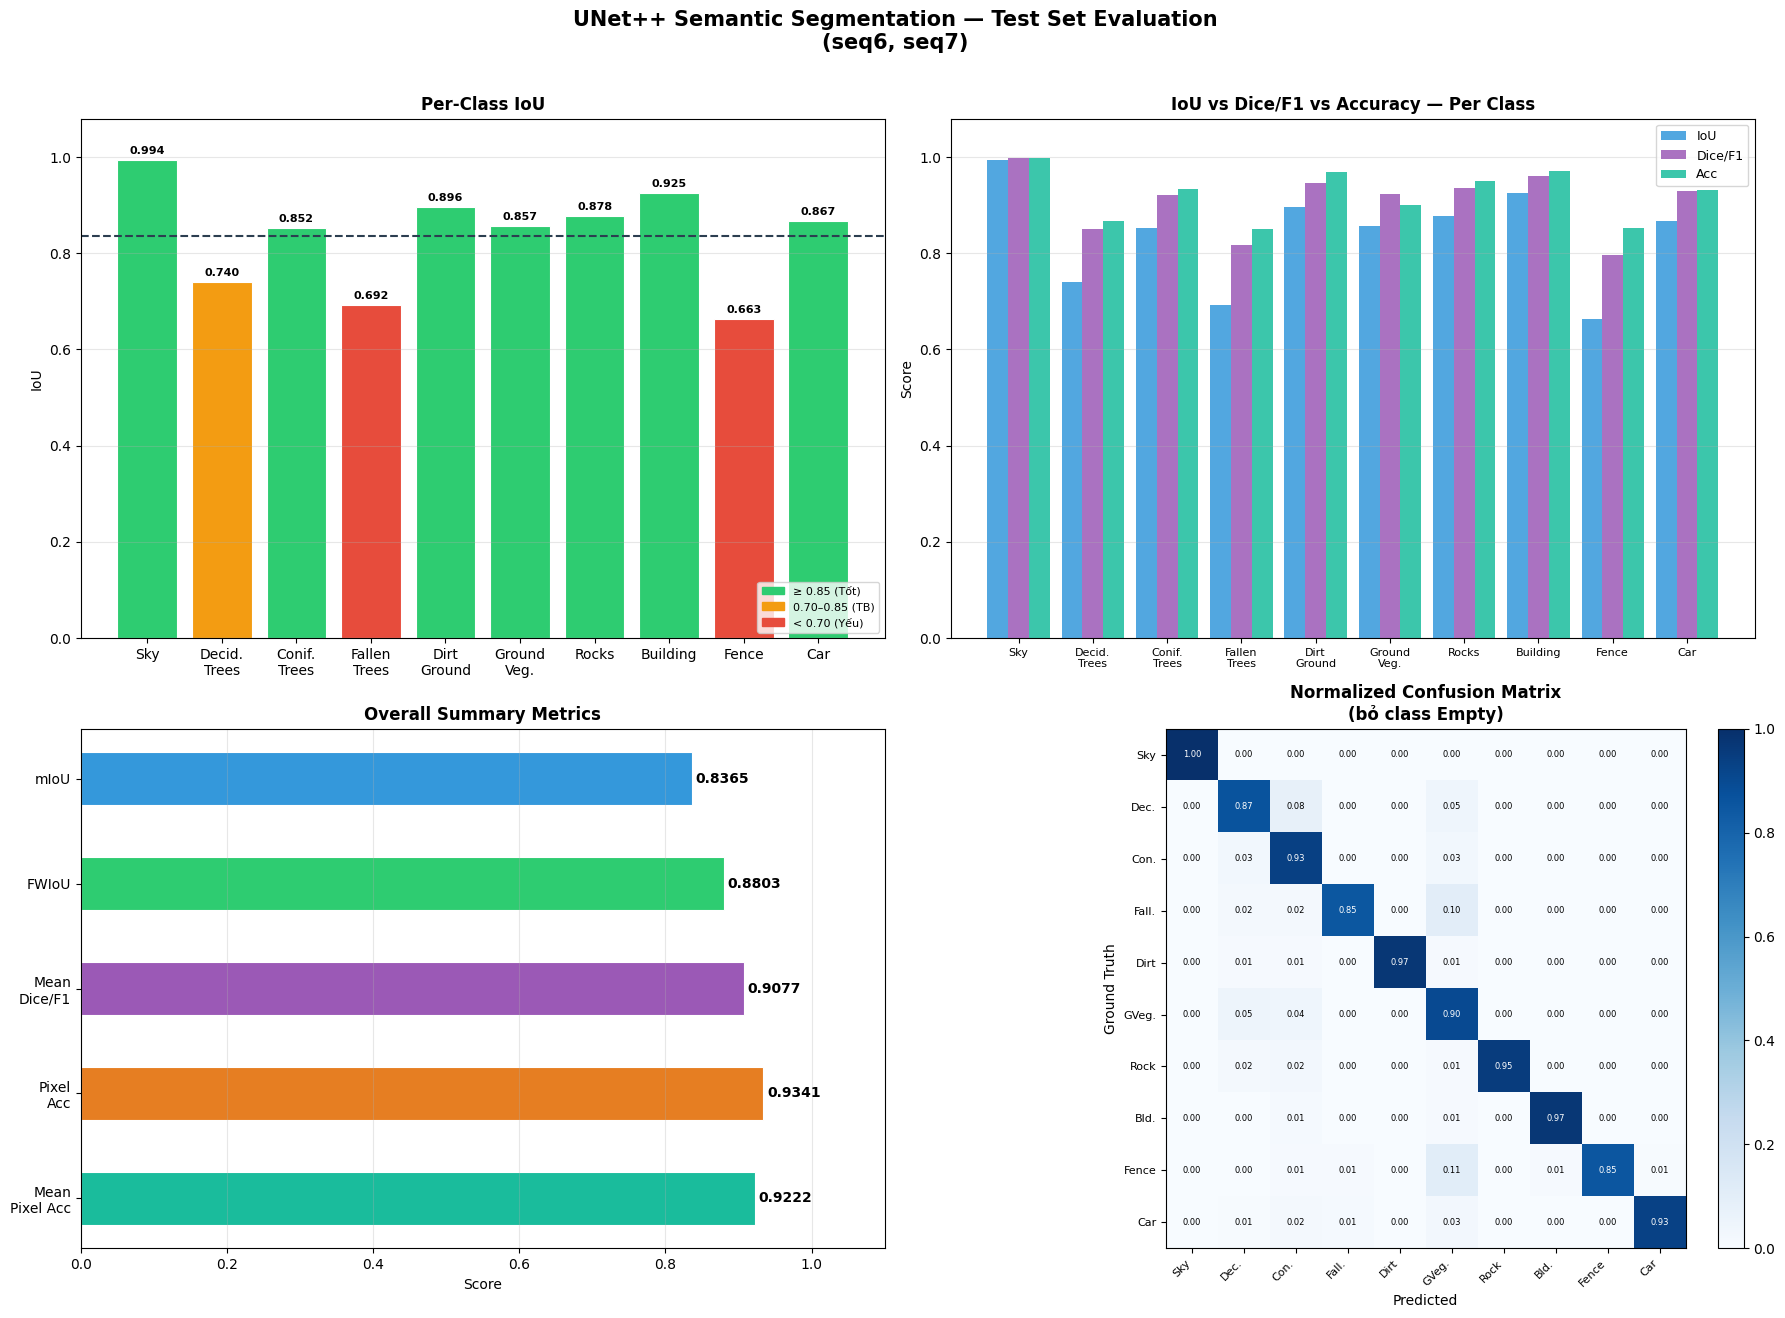
\includegraphics[width=\textwidth]{figures/fig_exp4_summary.png}
\caption{Tổng hợp đánh giá mô hình tốt nhất (Exp~4, adaptive) trên tập kiểm thử
(seq6, seq7): IoU theo lớp, so sánh IoU--Dice/F1--Accuracy, các chỉ số tổng thể
(mIoU $=0{,}8365$, FWIoU $=0{,}8803$, Pixel Acc $=0{,}9341$) và ma trận nhầm lẫn
chuẩn hóa.}
\label{fig:exp4_summary}
\end{figure}

\section{Kết quả theo từng lớp}
\label{sec:per_class}

Bảng~\ref{tab:perclass} là bằng chứng cốt lõi: IoU theo từng lớp cho thấy chính xác
chiến lược nào cải thiện lớp nào. Các lớp được sắp theo tần suất giảm dần; bốn lớp
hiếm ($<1\%$) được tô đậm.

\begin{table}[H]
\centering
\caption{IoU theo từng lớp trên tập kiểm thử (seq6, seq7).}
\label{tab:perclass}
\small
\begin{tabular}{l c c c c c}
\toprule
\textbf{Lớp} & \textbf{Tần suất} & \textbf{Exp1 CE} & \textbf{Exp2 CE+W} & \textbf{Exp3 FDC} & \textbf{Exp4 Adapt} \\
\midrule
Sky                & 20{,}33\% & 0{,}9940 & 0{,}9934 & 0{,}9936 & \textbf{0{,}9939} \\
Coniferous\_trees  & 27{,}85\% & \textbf{0{,}8550} & 0{,}8420 & 0{,}8454 & 0{,}8523 \\
Ground\_vegetation & 32{,}40\% & \textbf{0{,}8597} & 0{,}8475 & 0{,}8508 & 0{,}8570 \\
Deciduous\_trees   & 15{,}11\% & \textbf{0{,}7407} & 0{,}7235 & 0{,}7292 & 0{,}7404 \\
Dirt\_ground       & 1{,}83\%  & \textbf{0{,}8997} & 0{,}8890 & 0{,}8933 & 0{,}8959 \\
Rocks              & 1{,}74\%  & \textbf{0{,}8805} & 0{,}8634 & 0{,}8731 & 0{,}8782 \\
\textbf{Fallen\_trees} & \textbf{0{,}52\%} & 0{,}6706 & 0{,}6494 & 0{,}6711 & \textbf{0{,}6921} \\
\textbf{Building}  & \textbf{0{,}18\%}  & 0{,}9102 & 0{,}8729 & 0{,}9176 & \textbf{0{,}9252} \\
\textbf{Car}       & \textbf{0{,}04\%}  & 0{,}8232 & 0{,}8419 & 0{,}8545 & \textbf{0{,}8675} \\
\textbf{Fence}     & \textbf{0{,}01\%}  & 0{,}5535 & 0{,}6193 & 0{,}6413 & \textbf{0{,}6628} \\
\midrule
\textbf{mIoU}      &           & 0{,}8187 & 0{,}8142 & 0{,}8270 & \textbf{0{,}8365} \\
\bottomrule
\end{tabular}
\end{table}

\section{Phân tích trên các lớp hiếm}

Bảng~\ref{tab:rare} làm nổi bật mức cải thiện trên bốn lớp hiếm so với baseline.

\begin{table}[H]
\centering
\caption{Cải thiện IoU trên các lớp hiếm (so với Exp1, điểm phần trăm).}
\label{tab:rare}
\begin{tabular}{l c c c}
\toprule
\textbf{Lớp hiếm} & \textbf{Exp2 vs CE} & \textbf{Exp3 vs CE} & \textbf{Exp4 vs CE} \\
\midrule
Fence (0{,}01\%)        & $+6{,}58$ & $+8{,}78$ & \textbf{$+10{,}93$} \\
Car (0{,}04\%)          & $+1{,}87$ & $+3{,}13$ & \textbf{$+4{,}43$} \\
Building (0{,}18\%)     & $-3{,}73$ & $+0{,}74$ & \textbf{$+1{,}50$} \\
Fallen\_trees (0{,}52\%)& $-2{,}12$ & $+0{,}05$ & \textbf{$+2{,}15$} \\
\bottomrule
\end{tabular}
\end{table}

\noindent\textbf{Diễn giải:}
\begin{itemize}[leftmargin=1.4cm]
  \item \textbf{Exp 2 (CE+trọng số):} nâng được lớp cực hiếm (Fence $+6{,}6$,
  Car $+1{,}9$) nhưng \emph{làm hỏng} lớp Building ($-3{,}7$) và đa số các lớp phổ
  biến $\Rightarrow$ mIoU tổng giảm. Đây là dấu hiệu điển hình của over-weighting.
  \item \textbf{Exp 3 (Focal+Dice+CE):} cải thiện lớp hiếm mạnh hơn mà ít gây hại
  cho lớp phổ biến (nhờ Dice tối ưu vùng chồng lấp) $\Rightarrow$ mIoU tăng.
  \item \textbf{Exp 4 (thích nghi):} đạt mức cải thiện lớn nhất trên \emph{tất cả}
  lớp hiếm, đồng thời gần như khôi phục hiệu năng lớp phổ biến về mức baseline
  $\Rightarrow$ mIoU cao nhất. Trọng số học được giúp cân bằng tự động giữa các
  thành phần loss.
\end{itemize}

\begin{figure}[H]
\centering
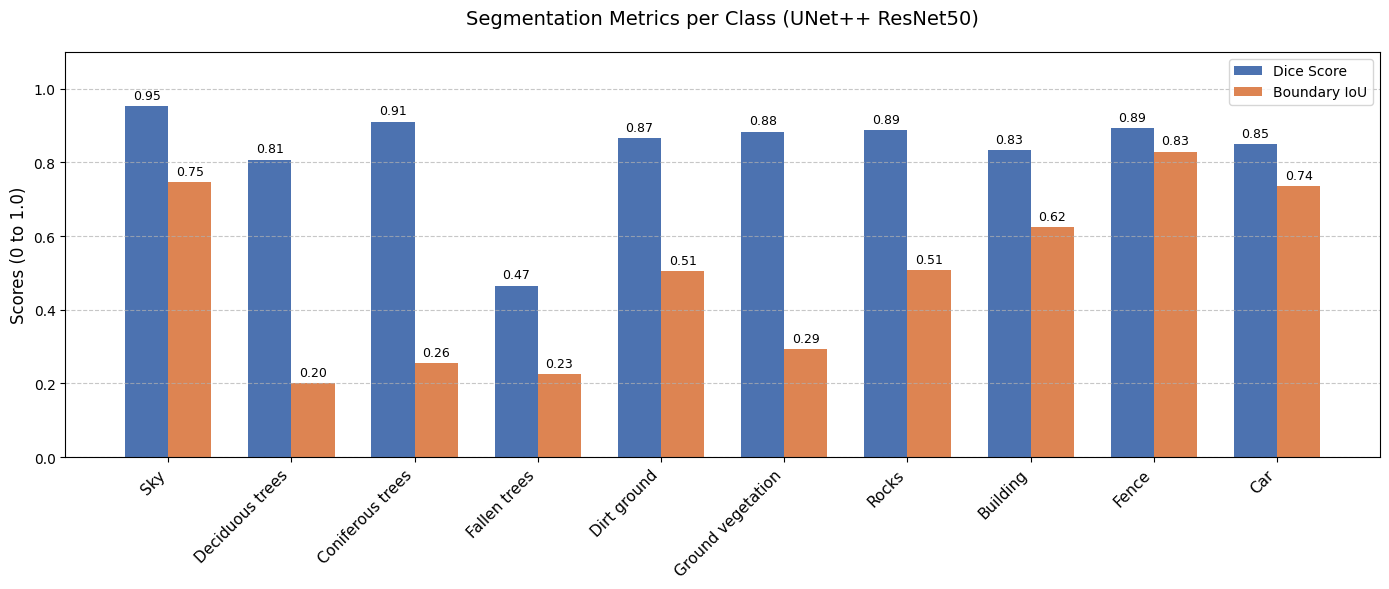
\includegraphics[width=\textwidth]{figures/fig_perclass_metrics.png}
\caption{Dice score và Boundary IoU theo từng lớp. Các lớp hiếm/nhỏ (Fallen trees,
Fence) có Boundary IoU thấp rõ rệt --- cho thấy khó khăn chủ yếu nằm ở vùng biên.}
\label{fig:perclass_metrics}
\end{figure}

\section{Diễn biến trọng số thích nghi (Exp 4)}

Trong Exp 4, ba trọng số $w_F, w_D, w_{CE}$ (suy ra từ $\sigma_k$ học được) thay đổi
theo epoch: khởi tạo $1{,}0$ và tăng dần trong các epoch đầu (ví dụ epoch~1:
$\approx 1{,}12/1{,}13/1{,}08$; epoch~3: $\approx 1{,}73/1{,}75/1{,}65$), cho thấy mô
hình tự điều chỉnh tỷ trọng giữa Focal, Dice và CE thay vì cố định thủ công. Giá trị
loss có thể âm do số hạng $\log\sigma_k$ (xem Mục~\ref{sec:adaptive}) --- hành vi
bình thường.

\HINH{Đường cong huấn luyện (loss \& mIoU) và diễn biến $w_F, w_D, w_{CE}$ theo epoch.}

\section{Kết quả định tính}

\begin{figure}[H]
\centering
\begin{subfigure}{0.48\textwidth}
  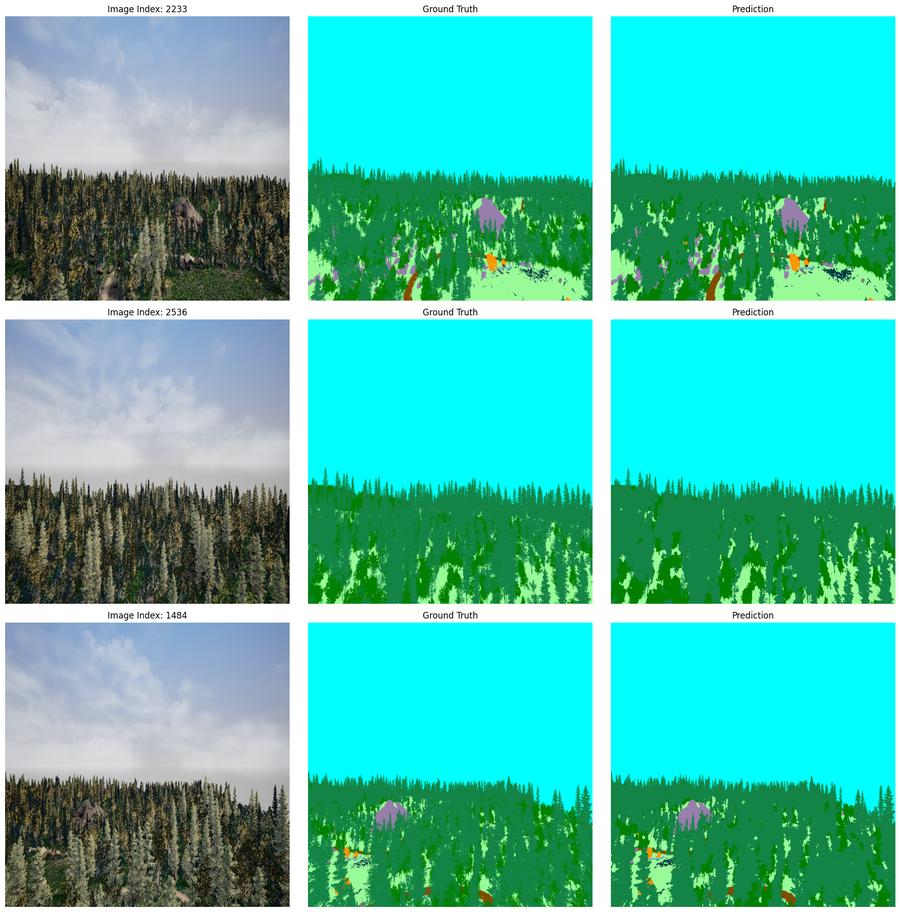
\includegraphics[width=\linewidth]{figures/qual_exp1.png}
  \caption{Exp 1 --- CE thuần}
\end{subfigure}\hfill
\begin{subfigure}{0.48\textwidth}
  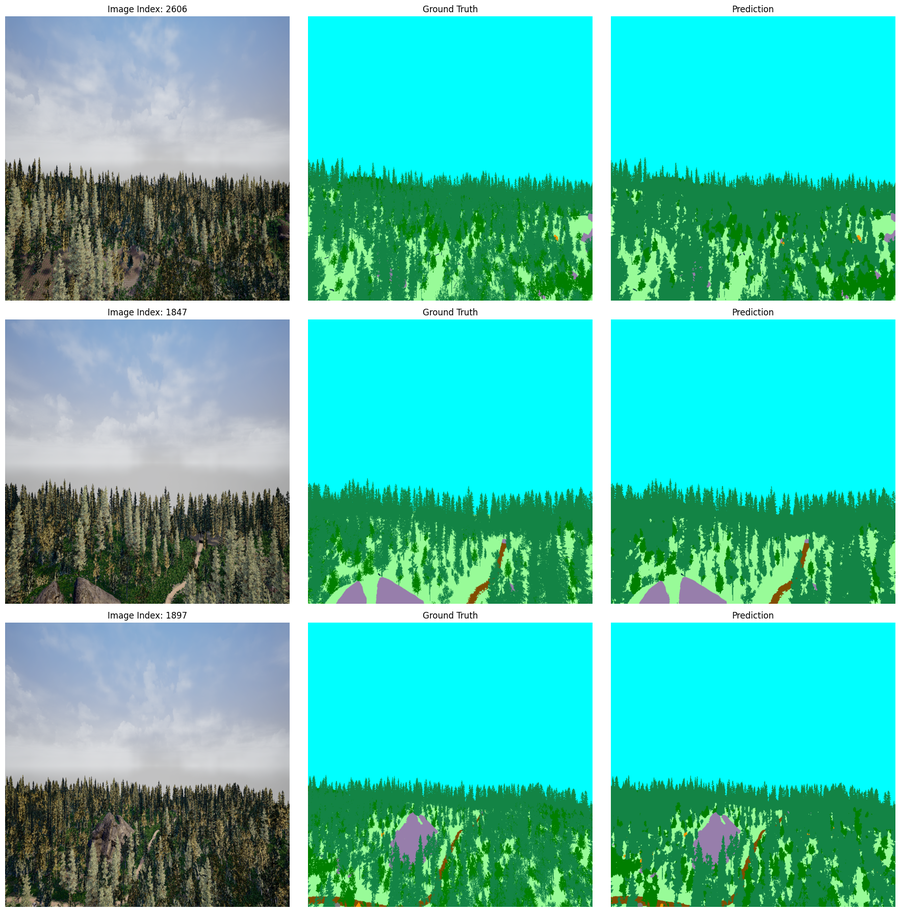
\includegraphics[width=\linewidth]{figures/qual_exp2.png}
  \caption{Exp 2 --- CE + trọng số}
\end{subfigure}

\vspace{4pt}
\begin{subfigure}{0.48\textwidth}
  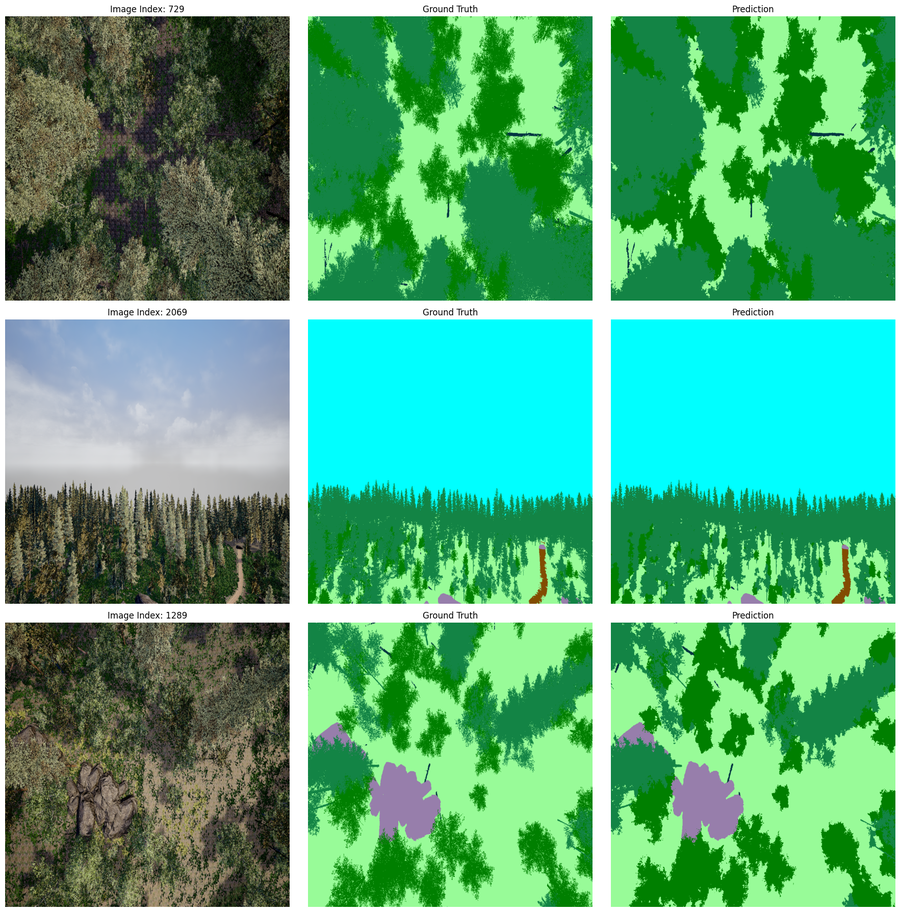
\includegraphics[width=\linewidth]{figures/qual_exp3.png}
  \caption{Exp 3 --- Focal+Dice+CE}
\end{subfigure}\hfill
\begin{subfigure}{0.48\textwidth}
  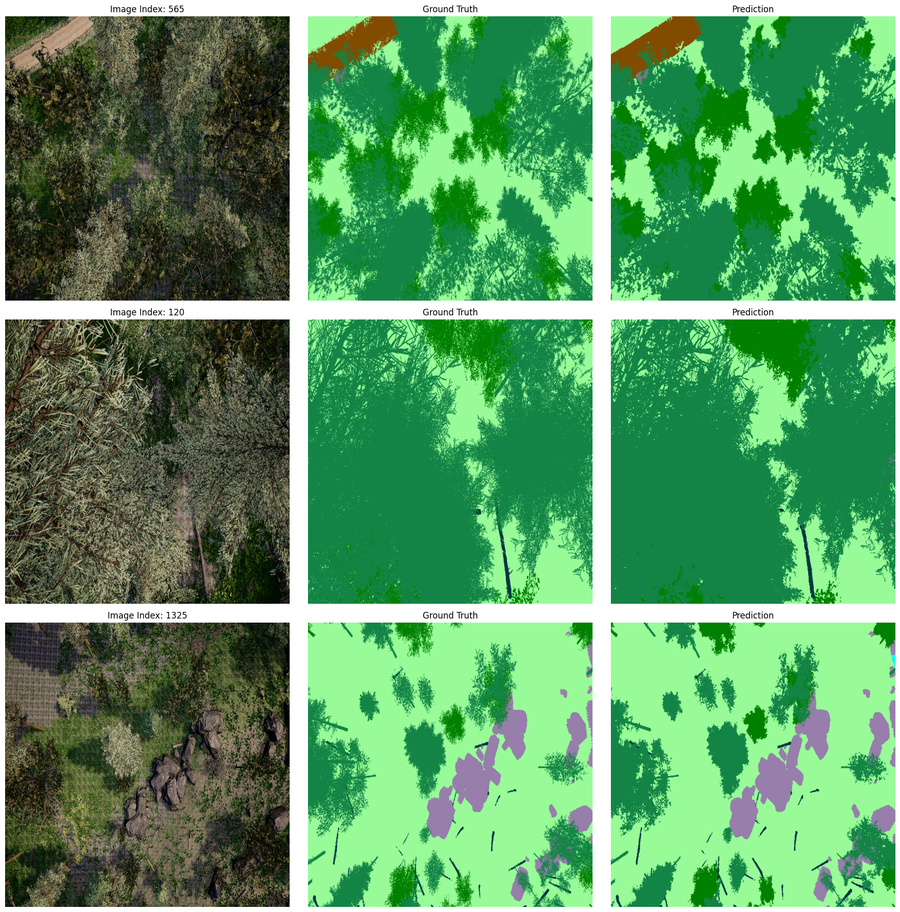
\includegraphics[width=\linewidth]{figures/qual_exp4.png}
  \caption{Exp 4 --- Adaptive}
\end{subfigure}
\caption{Kết quả định tính của bốn thí nghiệm trên tập kiểm thử (mỗi panel: 3 mẫu, cột
Ảnh gốc / Nhãn chuẩn / Dự đoán). \textit{Lưu ý:} các mẫu được chọn ngẫu nhiên độc lập
trong từng notebook nên không trùng nhau giữa các thí nghiệm.}
\label{fig:qual_montage}
\end{figure}

\TBD{Để so sánh trực tiếp công bằng: chạy lại inference của cả 4 mô hình trên CÙNG vài
chỉ số ảnh cố định, cắt cận cảnh vùng có Fence/Car, rồi thay hình ở trên.}

% =====================================================================
\section{Đánh giá độ bền theo điều kiện thời tiết \textnormal{(\TBD{đang tiến hành})}}
\label{sec:weather}

Để kiểm tra khả năng tổng quát hóa, mô hình tốt nhất (Exp 4) đang được đánh giá trên
các điều kiện ánh sáng/thời tiết khác nhau. Bảng~\ref{tab:weather} sẽ tổng hợp khi có
đủ kết quả.

\begin{table}[H]
\centering
\caption{mIoU theo điều kiện thời tiết (đánh giá chéo miền).}
\label{tab:weather}
\begin{tabular}{l c c c}
\toprule
\textbf{Điều kiện} & \textbf{Số ảnh} & \textbf{mIoU} & \textbf{Ghi chú} \\
\midrule
Sunny             & \TBD{} & \TBD{} & \TBD{} \\
Overcast          & \TBD{} & \TBD{} & \TBD{} \\
Sunny + Overcast  & \TBD{} & \TBD{} & \TBD{} \\
\bottomrule
\end{tabular}
\end{table}

\noindent\textit{Kết quả sơ bộ (một seed, chưa đầy đủ):} đánh giá chéo miền của mô
hình Exp 4 cho mIoU giảm đáng kể trên dữ liệu overcast ($\approx 0{,}55$) và dữ liệu
trộn ($\approx 0{,}59$--$0{,}72$), phản ánh domain gap về ánh sáng.
\TBD{Hoàn thiện và chuẩn hóa các phép đánh giá này; điền số chính thức vào bảng.}

% =====================================================================
\section{Đánh giá trên bộ dữ liệu WildUAV \textnormal{(\TBD{đang tiến hành})}}
\label{sec:wilduav}

Đánh giá trên bộ dữ liệu thực tế \textbf{WildUAV} nhằm kiểm tra khả năng chuyển miền
từ dữ liệu mô phỏng (AirSim) sang ảnh thực.

\begin{table}[H]
\centering
\caption{Kết quả trên WildUAV.}
\label{tab:wilduav}
\begin{tabular}{l c c c}
\toprule
\textbf{Mô hình / Loss} & \textbf{mIoU} & \textbf{PA} & \textbf{Ghi chú} \\
\midrule
Exp 4 (adaptive) & \TBD{} & \TBD{} & \TBD{ánh xạ lớp WildUAV $\leftrightarrow$ 11 lớp} \\
\bottomrule
\end{tabular}
\end{table}
\TBD{Bổ sung mô tả WildUAV (số ảnh, lớp, cách ánh xạ nhãn) và điền kết quả.}

% =====================================================================
\section{Mở rộng đa kiến trúc \textnormal{(\TBD{đang tiến hành})}}
\label{sec:multi_arch}

Ngoài UNet++/ResNet50, dự án hướng tới một \textbf{benchmark đa kiến trúc} (CNN,
Transformer, mô hình nhẹ) dùng hàm mất mát tốt nhất (adaptive), mỗi cấu hình chạy 3
seed để bảo đảm ý nghĩa thống kê. Bảng~\ref{tab:matrix} là ma trận thực nghiệm dự
kiến (25 cấu hình, chia 5 nhóm).

\begin{table}[H]
\centering
\caption{Ma trận thực nghiệm đa kiến trúc dự kiến (25 cấu hình $\times$ 3 seed).}
\label{tab:matrix}
\small
\begin{tabular}{c l l l}
\toprule
\textbf{Nhóm} & \textbf{Mục đích} & \textbf{Decoder} & \textbf{Encoder} \\
\midrule
A & CNN baseline      & UNet, DeepLabV3+, UNet++ & resnet34/50/101 \\
B & CNN hiện đại      & UNet, UPerNet, DeepLabV3+ & efficientnet, convnext, se\_resnet \\
C & Transformer       & SegFormer, UPerNet & mit\_b3/b5, swinv2, pvt\_v2 \\
D & Ablation decoder  & UNet/DLV3+/SegFormer/UPerNet/PSPNet/FPN & mit\_b3 (cố định) \\
E & HRNet \& nhẹ      & UNet, DeepLabV3+, Linknet & hrnet\_w48, mobilenet\_v2, mobileone \\
\bottomrule
\end{tabular}
\end{table}

Kết quả chính thức (cùng loss adaptive, cùng split, 3 seed) sẽ tổng hợp ở
Bảng~\ref{tab:multiarch}.

\begin{table}[H]
\centering
\caption{So sánh đa kiến trúc (cùng loss adaptive, cùng split, 3 seed).}
\label{tab:multiarch}
\small
\begin{tabular}{l l c c c c}
\toprule
\textbf{Decoder} & \textbf{Encoder} & \textbf{Test mIoU} & \textbf{Params} & \textbf{FLOPs} & \textbf{FPS} \\
\midrule
UNet++ & ResNet50 & 0{,}8365$^\dagger$ & 48{,}99M & 230{,}47G & 12{,}5 \\
\TBD{} & \TBD{} & \TBD{} & \TBD{} & \TBD{} & \TBD{} \\
\bottomrule
\end{tabular}
\end{table}
{\footnotesize $^\dagger$ một seed (2025), $1024\times1024$. Các dòng khác: \TBD{bổ sung}.}

\subsection*{Kết quả sơ bộ (split/cấu hình cũ --- chỉ để tham khảo)}
Trước nghiên cứu này, ba kiến trúc đã được đánh giá nhưng trên \textbf{split kiểm thử
khác} (seq9) và \textbf{cấu hình chưa đồng nhất} (kích thước ảnh, loss, patience khác
nhau), nên \textbf{không so sánh trực tiếp} được với các con số trong báo cáo:
SegFormer/MiT-B5 $\approx 0{,}703$; DeepLabV3+/MiT-B5 $\approx 0{,}683$;
UNet++/ResNet50 $\approx 0{,}605$. Các giá trị này gợi ý lợi thế của encoder
Transformer, và sẽ được chạy lại với cấu hình đồng nhất.
\TBD{Chạy lại 3 kiến trúc trên với loss adaptive + cùng split/cấu hình rồi điền vào
Bảng~\ref{tab:multiarch}.}

% =====================================================================
\section{Đánh giá nhiều seed (Exp 4) \textnormal{(\TBD{một phần})}}
\label{sec:multiseed}

Để đảm bảo ý nghĩa thống kê, Exp 4 cần chạy trên 3 seed. Hiện mới có seed 2025.

\begin{table}[H]
\centering
\caption{Exp 4 trên nhiều seed.}
\label{tab:seeds}
\begin{tabular}{c c}
\toprule
\textbf{Seed} & \textbf{Test mIoU} \\
\midrule
2025 & 0{,}8365 \\
42   & \TBD{} \\
123  & \TBD{} \\
\midrule
\textbf{Trung bình $\pm$ độ lệch} & \TBD{} \\
\bottomrule
\end{tabular}
\end{table}
\TBD{Chạy seed 42 và 123 cho Exp 4, điền giá trị và tính trung bình $\pm$ std.}

% ============================================================
\chapter{THẢO LUẬN}
\label{ch:thao_luan}
% ============================================================

\section{Vì sao trọng số lớp đơn thuần không hiệu quả?}

Kết quả Exp 2 ($-0{,}45$ pp so với baseline) thoạt nhìn nghịch lý, nhưng phù hợp với
lý thuyết. Trọng số nghịch tần suất nâng gradient của lớp hiếm lên rất cao
(Bảng~\ref{tab:imbalance}: Fence $= 7{,}22$, Car $= 2{,}03$), khiến mô hình "cố gắng"
dự đoán các lớp này ở cả những vùng không chắc chắn $\Rightarrow$ tăng dương tính giả
và \textbf{xâm lấn} sang lớp phổ biến. Quan sát trong Bảng~\ref{tab:perclass} xác
nhận: Fence/Car tăng nhưng Building, Deciduous, Coniferous, Rocks đều giảm. Tổng hợp
lại, phần mất ở lớp phổ biến lớn hơn phần được ở lớp hiếm, kéo mIoU xuống.

\section{Vì sao tổ hợp Focal+Dice+CE hiệu quả hơn?}

Hai cơ chế bổ trợ giải thích ưu thế của Exp 3 và Exp 4:
\begin{itemize}[leftmargin=1.4cm]
  \item \textbf{Focal Loss} tập trung vào điểm ảnh khó (biên, vật thể nhỏ) thay vì
  ép theo tần suất lớp, nên ít gây dương tính giả hơn trọng số cứng.
  \item \textbf{Dice Loss} tối ưu trực tiếp độ chồng lấp vùng và bất biến với kích
  thước lớp, giúp lớp nhỏ (Fence, Car) đóng góp tương xứng vào mục tiêu tối ưu mà
  không bóp méo lớp lớn.
\end{itemize}
Sự kết hợp này nâng lớp hiếm \emph{và} bảo toàn lớp phổ biến --- điều mà trọng số CE
đơn thuần không làm được.

\section{Giá trị của cơ chế thích nghi}

Exp 4 vượt trội nhờ \emph{học} tỷ trọng giữa ba thành phần loss thay vì cố định. Cơ
chế bất định đa nhiệm~\cite{kendall2018uncertainty} cho phép mô hình tự giảm ảnh
hưởng của thành phần "nhiễu" theo từng giai đoạn huấn luyện. Kết quả là Exp 4 đạt IoU
cao nhất trên \emph{toàn bộ} lớp hiếm đồng thời khôi phục gần như hoàn toàn hiệu năng
lớp phổ biến (xem Bảng~\ref{tab:perclass}).

\section{Phân tích lỗi vật thể nhỏ}

Phân tích chi tiết (recall, precision, nhầm lẫn) cho các lớp nhỏ cho thấy lỗi phổ
biến là \emph{nhầm sang Ground\_vegetation} --- lớp nền chiếm ưu thế. Ví dụ với
baseline, một phần đáng kể điểm ảnh Fence và Fallen\_trees bị gán nhầm thành
Ground\_vegetation. Các chiến lược Focal+Dice giảm đáng kể kiểu lỗi này.

\begin{figure}[H]
\centering
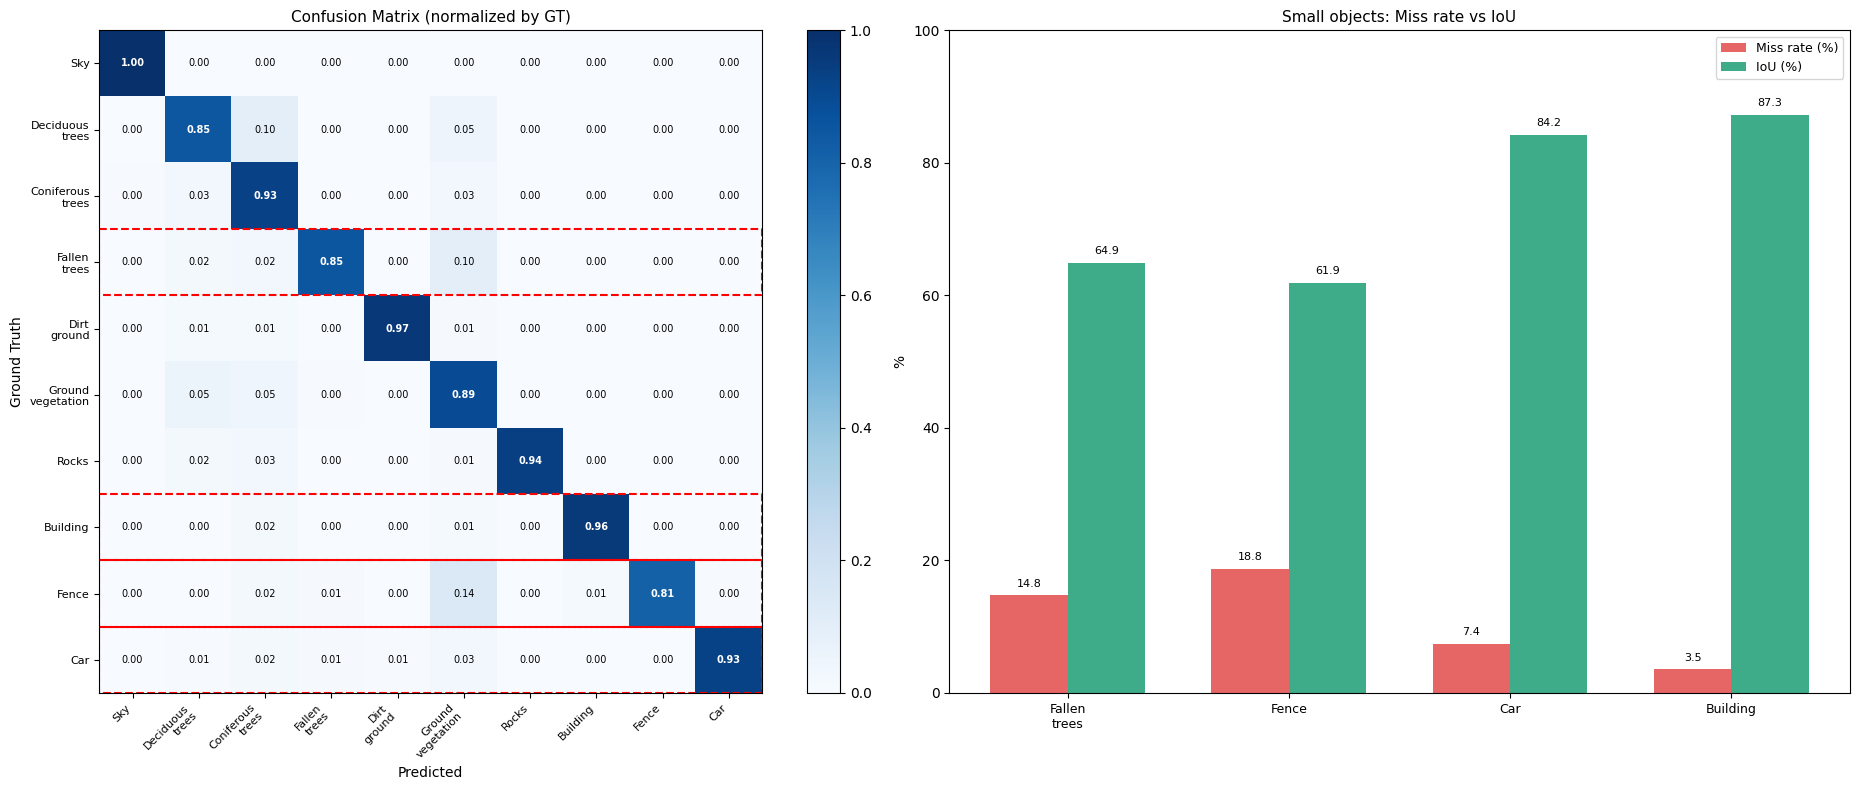
\includegraphics[width=\textwidth]{figures/fig_confusion_smallobj.png}
\caption{Trái: ma trận nhầm lẫn chuẩn hóa theo nhãn chuẩn (10 lớp). Phải: tỷ lệ bỏ
sót (miss rate) và IoU của bốn lớp nhỏ/hiếm. Lỗi phổ biến nhất là nhầm Fence và Fallen
trees sang Ground vegetation (cột tương ứng trong ma trận).}
\label{fig:confusion}
\end{figure}

\section{Hạn chế và mối đe dọa tới tính hợp lệ}
\label{sec:han_che}

Để bảo đảm tính nghiêm túc khoa học, báo cáo nêu rõ các hạn chế sau:

\begin{enumerate}[leftmargin=1.4cm]
  \item \textbf{Số epoch chưa đồng nhất.} Exp 4 huấn luyện 100 epoch trong khi Exp
  1--3 chỉ 50 epoch; một phần ưu thế của Exp 4 có thể đến từ thời gian huấn luyện dài
  hơn. \emph{Khắc phục:} chạy lại Exp 4 ở 50 epoch (hoặc Exp 1--3 ở 100 epoch) để so
  sánh tách bạch ảnh hưởng của loss.
  \item \textbf{Giao thức đánh giá chưa thống nhất.} Exp 1 và Exp 4 đánh giá bằng
  \emph{checkpoint tốt nhất}, còn Exp 2 và Exp 3 đánh giá bằng \emph{mô hình ở epoch
  cuối}. \emph{Khắc phục:} thống nhất dùng checkpoint tốt nhất cho cả bốn.
  \item \textbf{Mới một seed cho Exp 4.} Kết quả $0{,}8365$ là của seed 2025; cần
  bổ sung seed 42 và 123 để báo cáo trung bình $\pm$ độ lệch chuẩn
  (Mục~\ref{sec:multiseed}).
  \item \textbf{Cách chia dữ liệu đặc thù.} Tập kiểm thử \{seq6, seq7\} chứa chuỗi
  chụp ngang (nhiều Sky), khiến mIoU cao và không so trực tiếp được với benchmark
  dùng cách chia khác (Mục~\ref{sec:split}).
  \item \textbf{Dữ liệu mô phỏng.} Bộ dữ liệu sinh từ AirSim; khả năng tổng quát hóa
  sang ảnh thực cần kiểm chứng qua WildUAV (Mục~\ref{sec:wilduav}).
  \item \textbf{Một kiến trúc.} Kết luận giới hạn ở UNet++/ResNet50; cần xác nhận
  trên các kiến trúc khác (Mục~\ref{sec:multi_arch}).
\end{enumerate}

% ============================================================
\chapter{KẾT LUẬN VÀ HƯỚNG PHÁT TRIỂN}
\label{ch:ket_luan}
% ============================================================

\section{Kết luận}

Báo cáo đã nghiên cứu một cách hệ thống bốn chiến lược xử lý mất cân bằng lớp cho bài
toán phân đoạn ngữ nghĩa ảnh UAV rừng, trên cùng kiến trúc UNet++/ResNet50. Các kết
luận chính:

\begin{itemize}[leftmargin=1.4cm]
  \item Bộ dữ liệu rừng UAV có mức \textbf{mất cân bằng lớp rất nghiêm trọng}
  ($2.761\times$), với hai lớp cực hiếm Fence ($0{,}01\%$) và Car ($0{,}04\%$).
  \item \textbf{Trọng số lớp đơn thuần không phải giải pháp tốt}: tuy nâng được lớp
  hiếm nhưng làm giảm hiệu năng lớp phổ biến, dẫn tới mIoU tổng giảm
  ($0{,}8187 \rightarrow 0{,}8142$).
  \item \textbf{Tổ hợp Focal+Dice+CE} cải thiện ổn định ($0{,}8270$), và
  \textbf{phiên bản trọng số thích nghi cho kết quả tốt nhất} ($0{,}8365$,
  $+1{,}78$ pp so với baseline), đặc biệt trên các lớp hiếm (Fence $+10{,}9$ pp,
  Car $+4{,}4$ pp).
  \item Cơ chế \textbf{uncertainty weighting} cân bằng tự động các thành phần loss,
  vừa nâng lớp hiếm vừa bảo toàn lớp phổ biến --- là lựa chọn được khuyến nghị.
\end{itemize}

\section{Hướng phát triển}
\label{sec:huong_morong}

\begin{enumerate}[leftmargin=1.4cm]
  \item \textbf{Hoàn thiện tính chặt chẽ:} đồng nhất số epoch và giao thức đánh giá;
  bổ sung đủ 3 seed cho Exp 4 (Mục~\ref{sec:multiseed}).
  \item \textbf{Độ bền theo điều kiện thời tiết:} hoàn thiện đánh giá trên sunny,
  overcast và dữ liệu trộn (Mục~\ref{sec:weather}).
  \item \textbf{Chuyển miền sang ảnh thực:} đánh giá trên WildUAV
  (Mục~\ref{sec:wilduav}); cân nhắc kỹ thuật thích nghi miền (domain adaptation).
  \item \textbf{So sánh đa kiến trúc:} mở rộng sang CNN hiện đại (ConvNeXt,
  EfficientNetV2), Transformer (SegFormer, SwinV2) và mô hình nhẹ cho thiết bị biên
  (Mục~\ref{sec:multi_arch}).
  \item \textbf{Tăng cường dữ liệu \& hậu xử lý:} copy-paste cho lớp cực hiếm,
  Test-Time Augmentation, làm trơn biên (CRF).
\end{enumerate}


% ===================== TÀI LIỆU THAM KHẢO =====================
% ====================== TÀI LIỆU THAM KHẢO ======================
% Dùng thebibliography thủ công để biên dịch được ngay (không cần BibTeX/Biber).
% Nếu muốn dùng .bib, xem file refs.bib và chuyển sang biblatex.
\begin{thebibliography}{99}
\addcontentsline{toc}{chapter}{Tài liệu tham khảo}

\bibitem{long2015fcn}
J.~Long, E.~Shelhamer, and T.~Darrell,
``Fully Convolutional Networks for Semantic Segmentation,''
\textit{IEEE CVPR}, 2015, pp.~3431--3440.

\bibitem{ronneberger2015unet}
O.~Ronneberger, P.~Fischer, and T.~Brox,
``U-Net: Convolutional Networks for Biomedical Image Segmentation,''
\textit{MICCAI}, 2015, pp.~234--241.

\bibitem{zhou2018unetpp}
Z.~Zhou, M.~M.~R.~Siddiquee, N.~Tajbakhsh, and J.~Liang,
``UNet++: A Nested U-Net Architecture for Medical Image Segmentation,''
\textit{DLMIA/ML-CDS Workshop, MICCAI}, 2018.

\bibitem{he2016resnet}
K.~He, X.~Zhang, S.~Ren, and J.~Sun,
``Deep Residual Learning for Image Recognition,''
\textit{IEEE CVPR}, 2016, pp.~770--778.

\bibitem{chen2018deeplabv3plus}
L.-C.~Chen, Y.~Zhu, G.~Papandreou, F.~Schroff, and H.~Adam,
``Encoder-Decoder with Atrous Separable Convolution for Semantic Image
Segmentation,'' \textit{ECCV}, 2018, pp.~801--818.

\bibitem{xie2021segformer}
E.~Xie, W.~Wang, Z.~Yu, A.~Anandkumar, J.~M.~Alvarez, and P.~Luo,
``SegFormer: Simple and Efficient Design for Semantic Segmentation with
Transformers,'' \textit{NeurIPS}, 2021.

\bibitem{liu2021swin}
Z.~Liu, Y.~Lin, Y.~Cao, H.~Hu, Y.~Wei, Z.~Zhang, S.~Lin, and B.~Guo,
``Swin Transformer: Hierarchical Vision Transformer Using Shifted Windows,''
\textit{IEEE ICCV}, 2021, pp.~10012--10022.

\bibitem{liu2022convnext}
Z.~Liu, H.~Mao, C.-Y.~Wu, C.~Feichtenhofer, T.~Darrell, and S.~Xie,
``A ConvNet for the 2020s,'' \textit{IEEE CVPR}, 2022, pp.~11976--11986.

\bibitem{uavreview2024}
\textit{Methods and Datasets on Semantic Segmentation for Unmanned Aerial Vehicle
Remote Sensing Images: A Review,}
ISPRS Journal of Photogrammetry and Remote Sensing, 2024.
[Online]. \url{https://www.sciencedirect.com/science/article/abs/pii/S0924271624000844}

\bibitem{paszke2016enet}
A.~Paszke, A.~Chaurasia, S.~Kim, and E.~Culurciello,
``ENet: A Deep Neural Network Architecture for Real-Time Semantic Segmentation,''
\textit{arXiv:1606.02147}, 2016.

\bibitem{lin2017focal}
T.-Y.~Lin, P.~Goyal, R.~Girshick, K.~He, and P.~Doll\'ar,
``Focal Loss for Dense Object Detection,''
\textit{IEEE ICCV}, 2017, pp.~2980--2988.

\bibitem{milletari2016vnet}
F.~Milletari, N.~Navab, and S.-A.~Ahmadi,
``V-Net: Fully Convolutional Neural Networks for Volumetric Medical Image
Segmentation,''
\textit{3DV}, 2016, pp.~565--571.

\bibitem{sudre2017gdl}
C.~H.~Sudre, W.~Li, T.~Vercauteren, S.~Ourselin, and M.~J.~Cardoso,
``Generalised Dice Overlap as a Deep Learning Loss Function for Highly Unbalanced
Segmentations,''
\textit{DLMIA Workshop, MICCAI}, 2017, pp.~240--248.

\bibitem{salehi2017tversky}
S.~S.~M.~Salehi, D.~Erdogmus, and A.~Gholipour,
``Tversky Loss Function for Image Segmentation Using 3D Fully Convolutional Deep
Networks,'' \textit{MLMI Workshop, MICCAI}, 2017, pp.~379--387.

\bibitem{berman2018lovasz}
M.~Berman, A.~R.~Triki, and M.~B.~Blaschko,
``The Lovász-Softmax Loss: A Tractable Surrogate for the Optimization of the
Intersection-over-Union Measure in Neural Networks,''
\textit{IEEE CVPR}, 2018, pp.~4413--4421.

\bibitem{kendall2018uncertainty}
A.~Kendall, Y.~Gal, and R.~Cipolla,
``Multi-Task Learning Using Uncertainty to Weigh Losses for Scene Geometry and
Semantics,''
\textit{IEEE CVPR}, 2018, pp.~7482--7491.

\bibitem{jadon2020survey}
S.~Jadon,
``A Survey of Loss Functions for Semantic Segmentation,''
\textit{IEEE CIBCB}, 2020.

\bibitem{ma2021loss}
J.~Ma \textit{et al.},
``Loss Odyssey in Medical Image Segmentation,''
\textit{Medical Image Analysis}, vol.~71, 2021, art.~102035.

\bibitem{losssurvey2023}
R.~Azad \textit{et al.},
``Loss Functions in the Era of Semantic Segmentation: A Survey and Outlook,''
\textit{arXiv:2312.05391}, 2023.

\bibitem{deadwood2025}
``Using UAV Images and Deep Learning to Enhance the Mapping of Deadwood in Boreal
Forests,'' \textit{Remote Sensing of Environment}, 2025.
[Online]. \url{https://www.sciencedirect.com/science/article/pii/S0034425725003104}

\bibitem{fallentrees2021}
P.~Polewski \textit{et al.},
``Instance Segmentation of Fallen Trees in Aerial Color Infrared Imagery Using Active
Multi-Contour Evolution with FCN-Based Intensity Priors,''
\textit{arXiv:2105.01998}, 2021.

\bibitem{treeseg2024}
``Tree Semantic Segmentation from Aerial Image Time Series,''
\textit{arXiv:2407.13102}, 2024.

\bibitem{forestsemantic2024}
``ForestSemantic: A Dataset for Semantic Learning of Forest from Close-Range Sensing,''
\textit{Geo-spatial Information Science}, 2024.

\bibitem{forestdataset}
``Forest Inspection Dataset: A Synthetic UAV Dataset for Semantic Segmentation of
Forest Environments,'' \textit{Scientific Data}, Nature, 2026.
[Online]. \url{https://www.nature.com/articles/s41597-026-06665-x}.
Dữ liệu: Zenodo record~15511426, \url{https://zenodo.org/records/15511426}.
\TBD{kiểm tra lại tên tác giả/năm chính thức của bài báo dataset}

\TBD{Bổ sung các tham khảo về WildUAV và các kiến trúc so sánh khi hoàn thiện
Chương~\ref{ch:ket_qua}.}

\end{thebibliography}


% ===================== PHỤ LỤC =====================
\appendix
% ====================== PHỤ LỤC ======================
\chapter{Tái lập thực nghiệm}
\label{ap:reproduce}

\section*{A.1. Danh sách notebook}
Các notebook đã chạy (kèm số liệu) đặt trong \texttt{notebooks/executed/}:
\begin{itemize}[leftmargin=1.4cm]
  \item \texttt{exp1\_ce\_only.ipynb} --- Exp 1 (CE thuần), test mIoU $= 0{,}8187$.
  \item \texttt{exp2\_ce\_class\_weights.ipynb} --- Exp 2 (CE + trọng số),
  test mIoU $= 0{,}8142$.
  \item \texttt{exp3\_focal\_dice\_ce\_fixed.ipynb} --- Exp 3 (Focal+Dice+CE cố
  định), test mIoU $= 0{,}8270$.
  \item \texttt{exp4\_adaptive\_focal\_dice\_seed2025.ipynb} --- Exp 4 (thích nghi,
  seed 2025), test mIoU $= 0{,}8365$.
\end{itemize}

\section*{A.2. Bảng màu 11 lớp}
\begin{center}
\small
\begin{tabular}{c l l}
\toprule
\textbf{ID} & \textbf{Lớp} & \textbf{Màu (R,G,B)} \\
\midrule
0  & Sky               & (0, 255, 255) \\
1  & Deciduous\_trees  & (0, 127, 0) \\
2  & Coniferous\_trees & (19, 132, 69) \\
3  & Fallen\_trees     & (0, 53, 65) \\
4  & Dirt\_ground      & (130, 76, 0) \\
5  & Ground\_vegetation& (152, 251, 152) \\
6  & Rocks             & (151, 126, 171) \\
7  & Building          & (250, 150, 0) \\
8  & Fence             & (115, 176, 195) \\
9  & Car               & (123, 123, 123) \\
10 & Empty             & (0, 0, 0) \\
\bottomrule
\end{tabular}
\end{center}

\section*{A.3. Công thức trọng số lớp}
Trọng số tính theo công thức ENet (PT.~\ref{eq:enet_w}) với $\kappa = 1{,}02$ trên
tần suất tập huấn luyện.

\section*{A.4. Cấu trúc mã nguồn (\texttt{src/})}
\begin{center}
\small
\begin{tabular}{l l}
\toprule
\textbf{Module} & \textbf{Chức năng} \\
\midrule
\texttt{src/data/}       & \texttt{dataset.py}, \texttt{splits.py}, \texttt{transforms.py} --- nạp dữ liệu, chia tập, tăng cường \\
\texttt{src/models/}     & \texttt{unet.py}, \texttt{hrnet.py}, \texttt{pointflow.py} --- định nghĩa mô hình \\
\texttt{src/training/}   & \texttt{losses.py}, \texttt{metrics.py}, \texttt{trainer.py} --- hàm mất mát, độ đo, vòng huấn luyện \\
\texttt{src/evaluation/} & \texttt{evaluator.py}, \texttt{visualize.py}, \texttt{deforestation.py} --- đánh giá, trực quan hóa \\
\texttt{src/utils/}      & \texttt{config.py}, \texttt{logger.py} --- cấu hình, ghi log \\
\bottomrule
\end{tabular}
\end{center}

\section*{A.5. Pipeline 4 notebook}
\begin{center}
\small
\begin{tabular}{l c c l}
\toprule
\textbf{Notebook} & \textbf{Internet} & \textbf{GPU} & \textbf{Vai trò} \\
\midrule
NB01 & ON  & OFF & Chuẩn bị gói + trọng số pretrained (offline assets) \\
NB02 & OFF & ON  & Huấn luyện, lưu top-$k$ checkpoint \\
NB03 & ON  & ON  & Đánh giá tập kiểm thử, xuất \texttt{results\_all.csv} \\
NB04 & OFF & OFF & Tổng hợp bảng + hình cho báo cáo \\
\bottomrule
\end{tabular}
\end{center}

\TBD{Bổ sung: phiên bản thư viện, lệnh chạy, và liên kết tải checkpoint nếu công bố.}


\end{document}
